
%%%%%%%%%%%%%%%%%%%%%%%%%%%%%%%%%%%%%%%%%%%%%%%%%%%%%%%%%%%%%%%%%%%%%%%%%%%%%
\chapt[chap:ml]{Machine Learning}
\markboth{Machine Learning}{Machine Learning}
%%%%%%%%%%%%%%%%%%%%%%%%%%%%%%%%%%%%%%%%%%%%%%%%%%%%%%%%%%%%%%%%%%%%%%%%%%%%%


This \chapthing\ describes older machine learning PRs available in
GATE. The most up to date and best supported machine learning PR in
GATE is the \textbf{Learning Framework}. This is available on Github
at the address below:

https://github.com/GateNLP/gateplugin-LearningFramework

The two historical PRs described in this chapter are as follows:

\begin{itemize}

\item{The \textbf{Batch Learning PR} (in the \textbf{Learning} plugin) is targetted at NLP tasks including text classification, chunk learning (e.g. for
named entity recognition) and relation learning. It integrates LibSVM
for improved speed, along with the PAUM algorithm. It also offers a
Weka interface. It is documented in
Section~\ref{sec:ml:batch-learning-pr}.}
%It is introduced briefly
%in section~\ref{sect:learning-pr} and documented more fully in
%\Chapthing~\ref{chap:ml}. \Chapthing~\ref{chap:ml} also provides a
%short introduction to machine learning, in which concepts are defined.}

\item{The \textbf{Machine Learning PR} (in the \textbf{Machine\_Learning} plugin)
is GATE's even older machine learning offering. It offers wrappers for
Maxent, Weka and SVM Light. It is documented in
Section~\ref{sec:ml:machine-learning-pr}.}

\end{itemize}

To use GATE in conjunction with machine learning technologies that are
not supported by a GATE PR, you would need to export your data from
GATE to use with the ML technology outside of GATE. One possibility
for doing that would be to use the \textbf{Configurable Exporter PR}
described in
Section~\ref{sec:misc-creole:confexport}. The \textbf{Batch Learning
PR} also offers data export functionality.

The rest of the \chapthing\ is organised as follows. Section
\ref{sec:ml:generalities} introduces machine learning in general, focusing on the
terminology used and the meaning of the terms within GATE. We then move on to
describe the two Machine Learning processing resources, beginning with the Batch
Learning PR in Section~\ref{sec:ml:batch-learning-pr}. Section
\ref{sec:ml:batch-conf} describes all the configuration settings of the Batch
Learning PR one by one; i.e. all the elements in the configuration file for
setting the Batch Learning PR (the learning algorithm to be used and the options
for learning) and defining the NLP features for the problem. Section
\ref{sec:ml:batch-case-studies} presents three case studies with example
configuration files for the three types of NLP learning problems. Section
\ref{sec:ml:howto} lists the steps involved in using the Batch Learning PR.
Finally, Section \ref{sec:ml:batch-output} explains the outputs of the Batch
Learning PR for the four usage modes; namely training, application, evaluation
and producing feature files only, and in particular, the format of the feature
files and label list file produced by the Batch Learning PR.
Section~\ref{sec:ml:machine-learning-pr} outlines the original Machine Learning
PR in GATE.

%%%%%%%%%%%%%%%%%%%%%%%%%%%%%%%%%%%%%%%%%%%%%%%%%%%%%%%%%%%%%%%%%%%%%%%%%%%%%
\sect[sec:ml:generalities]{ML Generalities}
%%%%%%%%%%%%%%%%%%%%%%%%%%%%%%%%%%%%%%%%%%%%%%%%%%%%%%%%%%%%%%%%%%%%%%%%%%%%%

There are two main types of ML; supervised learning and unsupervised learning.
Supervised learning is more effective and much more widely used in NLP.
Classification is a particular example of supervised learning, in which the set
of training examples is split into multiple subsets (classes) and the algorithm
attempts to distribute new examples into the existing classes. This is the type
of ML that is used in GATE, and all further references to ML actually refer to
classification.

An ML algorithm `learns' about a phenomenon by looking at a set of occurrences
of that phenomenon that are used as examples. Based on these, a model is built
that can be used to predict characteristics of future (unseen) examples of the
phenomenon.

An ML implementation has two modes of functioning: training and application.  The
training phase consists of building a model (e.g. a statistical model, a decision
tree, a rule set, etc.) from a dataset of already classified instances.  During
application, the model built during training is used to classify new instances.


%The ML plugin in GATE is designed particularly for NLP learning. It can be used
%for the following three types of learning; text classification, chunk
%recognition, and relation extraction. These broadly cover NLP learning tasks.

Machine Learning in NLP falls broadly into three categories of task type; text
classification, chunk recognition, and relation extraction

\begin{itemize}
  
\item {\bf Text classification}
classifies text into pre-defined categories. The process can be
equally well applied at the document, sentence or token level. Typical
examples of text classification might be document classification,
opinionated sentence recognition, POS tagging of tokens and word sense
disambiguation.

\item {\bf Chunk recognition} often consists of two steps. First, it identifies
the chunks of interest in the text. It then assigns a label or labels to these
chunks. However some problems comprise simply the first step; identifying the
relevant chunks. Examples of chunk recognition include named entity recognition
(and more generally, information extraction), NP chunking and Chinese word
segmentation.

\item {\bf Relation extraction} determines whether or not a pair of terms in the
text has some type(s) of pre-defined relations. Two examples are named entity
relation extraction and co-reference resolution.

\end{itemize}

Typically, the three types of NLP learning use different linguistic features and
feature representations. For example, it has been recognised that for text
classification the so-called $tf-idf$ representation of n-grams is very effective
(e.g. with SVM).  For chunk recognition, identifying the start token and the end
token of the chunk by using the linguistic features of the token itself and the
surrounding tokens is effective and efficient. Relation extraction benefits from
both the linguistic features from each of the two terms involved in the relation
and the features of the two terms combined.

%The ML plugin implements suitable feature representations for the three types
%of NLP learning introduced above. It also implements or wraps the most widely
%used ML algorithms, including SVM, KNN, Naive Bayes, and the decision tree
%algorithm C4.5.  In addition, given a document set, it can produce feature
%vector files for export. Users therefore can use the feature files for
%evaluating learning algorithms of their own, for NLP learning tasks or for any
%other further processing.

The rest of this section explains some basic definitions in ML and
their specification in the ML plugin.

%%%%%%%%%%%%%%%%%%%%%%%%%%%%%%%%%%%%%%%%%%%%%%%%%%%%%%%%%%%%%%%%%%%%%%%%%%%%%
\subsect{Some Definitions}
%%%%%%%%%%%%%%%%%%%%%%%%%%%%%%%%%%%%%%%%%%%%%%%%%%%%%%%%%%%%%%%%%%%%%%%%%%%%%

\begin{itemize}
  
\item \textbf{instance}: an example of the studied phenomenon. An ML
algorithm learns a model from a set of known instances, called a
(training) dataset. It can then apply the learned model to another
(application) dataset.

\item \textbf{attribute}: a characteristic of the instances. Each instance is
defined by the values of its attributes. The set of possible attributes is well
defined and is the same for all instances in the training and application
datasets. `Feature' is also often used. However, in this context, this can
cause confusion with GATE annotation features.

\item \textbf{class}: an attribute for which the values are available in the
  training dataset for learning, but which are not present in the application
  dataset. ML is used to find the value of this attribute in the application
  dataset.

\end{itemize}

%%%%%%%%%%%%%%%%%%%%%%%%%%%%%%%%%%%%%%%%%%%%%%%%%%%%%%%%%%%%%%%%%%%%%%%%%%%%%
\subsect{GATE-Specific Interpretation of the Above Definitions}
%%%%%%%%%%%%%%%%%%%%%%%%%%%%%%%%%%%%%%%%%%%%%%%%%%%%%%%%%%%%%%%%%%%%%%%%%%%%%

\begin{itemize}

\item \textbf{instance}: an annotation. In order to use ML in GATE, users will
need to choose the type of annotations used as instances. Token annotations are a
good candidate for many NLP learning tasks such as information extraction and POS
tagging, but any type of annotation could be used (e.g. things that were found by
a previously run JAPE grammar, such as sentence annotations and document
annotations for sentence and document classification respectively).

\item \textbf{attribute}: an attribute is the value of a named feature of a
particular annotation type, which can either (partially) cover the instance
annotation considered or another instance annotation which is related to the
instance annotation considered.  The value of the attribute can refer to the
current instance or to an instance either situated at a specified location
relative to the current instance or having special relation with the current
instance.

\item \textbf{class}: any attribute referring to the current instance can be
marked as class attribute.

\end{itemize}

%There are ML algorithms which permit the incremental building of the
%model (e.g. the Updateable Classifiers in the WEKA library). These
%classifiers do not require the entire training dataset to build a
%model; the model improves with each new training instance that the
%algorithm is provided with.


%%%%%%%%%%%%%%%%%%%%%%%%%%%%%%%%%%%%%%%%%%%%%%%%%%%%%%%%%%%%%%%%%%%%%%%%%%%%%
\sect[sec:ml:batch-learning-pr]{Batch Learning PR}
%%%%%%%%%%%%%%%%%%%%%%%%%%%%%%%%%%%%%%%%%%%%%%%%%%%%%%%%%%%%%%%%%%%%%%%%%%%%%

This section describes the newest machine learning PR in GATE. The
implementation focuses on the three main types of learning in
NLP, namely chunk recognition (e.g. named entity recognition), text
classification and relation extraction.  The implementation for chunk
recognition is based on our work using support vector machines (SVM)
for information extraction \cite{Yaoyong05}. The text classification
is based on our work on opinionated sentence classification and patent
document classification (see \cite{Yaoyong07c} and \cite{Yaoyong07b},
respectively). The relation extraction is based on our work on named
entity relation extraction \cite{Wang06}.

The Batch Learning PR, given a set of documents, can also produce feature
files, containing linguistic features and feature vectors, and labels if there
are any in the documents. It can also produce document-term matrices and n-gram
based language models. Feature files are in text format and can be used outside
of GATE. Hence, users can use GATE-produced feature files off-line, for their own
purpose, e.g. evaluating new learning algorithms.

The PR also provides facilities for active learning, based
on support vector machines (SVM), mainly ranking the unlabelled
documents according to the confidence scores of the current SVM models
for those documents.

The primary learning algorithm implemented is SVM, which has achieved state of
the art performances for many NLP learning tasks. The training of SVM uses a
Java version of the SVM package LibSVM \cite{CC01a}. Application of SVM is
implemented by ourselves. The PAUM (Perceptron Algorithm with Uneven Margins)
is also included \cite{Yaoyong02a}, and on our test datasets has consistently
produced a performance to rival the SVM with much reduced training
times. Moreover, the ML implementation provides an interface to the
open-source machine learning package Weka \cite{Weka}, and can use machine
learning algorithms implemented in Weka. Three widely-used learning algorithms
are available in the current implementation: Naive Bayes, KNN and the C4.5
decision tree algorithm.

Access to ML implementations is provided in GATE by the `Batch Learning PR' (in
the `learning' plugin). The PR handles training and application of an ML model,
evaluation of learning on GATE documents, producing feature files and
ranking documents for Active Learning. It also makes it possible to view the
primal forms of a linear SVM. This PR is a Language Analyser so it can be used in
all default types of GATE controllers.

In order to use the Batch Learning processing resource, the user has to do
three things. First, the user has to annotate some training documents with the
labels that s/he wants the learning system to annotate in new documents. Those
label annotations should be GATE annotations. Secondly, the user may need to
pre-process the documents to obtain linguistic features for the learning.
Again, these features should be in the form of GATE annotations. GATE's plugin
ANNIE might be helpful for producing the linguistic features. Other resources
such as the NP Chunker and parser may also be helpful. By providing the
machine learning algorithm with more and better information on which to base
learning, chances of a good result are increased, so this preprocessing
stage is important. Finally the user has to create a configuration file for
setting the ML PR, e.g.  selecting the learning algorithm and defining the
linguistic features used in learning. Three example configuration files are
presented in this section; it might be helpful to take one of them as a
starting point and modify it.

%%%%%%%%%%%%%%%%%%%%%%%%%%%%%%%%%%%%%%%%%%%%%%%%%%%%%%%%%%%%%%%%%%%%%%%%%%%%%
\subsect[sec:ml:batch-conf]{Batch Learning PR Configuration File Settings}
%%%%%%%%%%%%%%%%%%%%%%%%%%%%%%%%%%%%%%%%%%%%%%%%%%%%%%%%%%%%%%%%%%%%%%%%%%%%%

In order to allow for more flexibility, all configuration parameters for the
PR are set through one external XML file, except for the learning mode, which
is selected through normal PR parameterisation. The XML file contains both the
configuration parameters of the Batch Learning PR itself and of the linguistic
data (namely the definitions of the instance and attributes) used by the Batch
Learning PR. The XML file is specified when creating a new Batch Learning PR.

The parent directory of the XML configuration file becomes the working directory.
A subdirectory in the working directory, named `savedFiles', will be created
(if it does not already exist). All the files produced by the Batch Learning PR,
including the NLP features files, label list file, feature vector file and
learned model file, will be stored in that subdirectory. A log file recording the
learning session is also created in this directory.

Below, we first describe the parameters of the Batch Learning PR. Then we explain
those settings specified in the configuration file.

 %in Appendix \ref{chap:mlconfig}.

%%%%%%%%%%%%%%%%%%%%%%%%%%%%%%%%%%%%%%%%%%%%%%%%%%%%%%%%%%%%%%%%%%%%%%%%%%%%%
\subsubsect[sec:ml:batch-not-conf]{PR Parameters: Settings not Specified in the
Configuration File}
%%%%%%%%%%%%%%%%%%%%%%%%%%%%%%%%%%%%%%%%%%%%%%%%%%%%%%%%%%%%%%%%%%%%%%%%%%%%%

For the sake of convenience, a few settings are not specified in the
configuration file. Instead the user should specify them as initialization or
run-time parameters of the PR, as in other PRs.

\begin{itemize}

\item {\bf URL (or path and name) of the configuration file}. The user is
required to give the URL of the configuration file when creating the PR. The
configuration file should be in XML format with the extension name {\em .xml}. It
contains most of learning settings and will be explained in detail in the next
subsection.

\item {\bf Corpus}. This is a run-time parameter, meaning that the user should
  specify it after creating the PR, and may change it between runs. The corpus
  contains the documents that the PR will use as learning data (training or
  application). For application, the documents should include all the
  annotations specified in the configuration file, except the class
  attribute. The annotations for class attribute should be available in the
  documents used for training or evaluation.

\item {\bf inputASName} is the annotation set containing the annotations for 
the linguistic features to be used and the class labels.

\item {\bf outputASName} is the annotation set in which the results
 of applying the models will be put. Note that it should be set the
same as the {\em inputASName} when doing the evaluation (i.e. setting the {\em
learningMode} as `EVALUATION').

\item {\bf learningMode} is a run-time parameter. It can be set as one of the
following values, `TRAINING', `APPLICATION', `EVALUATION',
`ProduceFeatureFilesOnly', `MITRAINING', `VIEWPRIMALFORMMODELS' and
`RankingDocsForAL'. The default learning mode is `TRAINING'.

\begin{itemize}

\item In {\bf TRAINING} mode, the PR learns from the data provided and saves the
models into a file called `learnedModels.save' under the sub-directory
`savedFiles' of the working directory.

\item If the user wants to apply the learned model to the data, s/he should
select {\bf APPLICATION} mode.
 In application mode, the PR reads the learned model from the file
 `learnedModels.save' in the subdirectory `savedFiles' and then applies the
 model to the data.

\item In {\bf EVALUATION} mode, the PR will do k-fold or hold-out test set
evaluation on the corpus provided (the method of the evaluation is specified in
the configuration file, see below), and output the evaluation results to the
messages window of GATE Developer, or standard out when using GATE Embedded, and
into the log file. When using evaluation mode, please make sure that the {\em
outputASName} is set to the same annotation set as the {\em inputASName}.

\item If the user only wants to produce feature data and feature vectors but does
not want to train or apply a model, s/he may select the {\bf
ProduceFeatureFilesOnly} mode. The feature files that the PR produces will be
explained in detail in Section \ref{sec:ml:feature}.

\item In {\bf MITRAINING} (mixed initiative training) mode, the training data are
appended to the end of any existing feature file. In contrast, in training mode,
the training data created in the current session overwrite any existing feature
file. Consequently, mixed initiative training mode uses both the training data
obtained in this session and the data that existed in the feature file before
starting the session. Hence, training mode is for batch learning, while mixed
initiative training mode can be used for on-line (or adaptive, or
mixed-initiative) learning. There is one parameter for mixed initiative training
mode specifying the minimal number of newly added documents before starting the
learning procedure to update the learned model. The parameter can be defined in
the configuration file.

\item {\bf VIEWPRIMALFORMMODELS} mode is used for displaying the most salient
NLP features in the learned models. In the current implementation, the mode is only
valid with the linear SVM model, in which the most salient NLP features
correspond to the biggest (absolute values of) weights in the weight vector. In
the configuration file one can specify two parameters to determine the number of
displayed NLP features for positive and negative weights. Note that if e.g. the
number for negative weight is set as $0$, then no NLP feature is displayed for
negative weights.

\item {\bf RankingDocsForAL} applies the current learned SVM models (in the
sub-directory `savedFiles') to the feature vectors stored in the file
`fvsDataSelecting.save' in the sub-directory `savedFiles' and ranks the
documents according to the margins of the examples in one document to the SVM
models. The ranked list of documents will be put into the file
`ALRankedDocs.save'.

\end{itemize}

\item {\bf runProtocolDir}: if specified, the URL of a directory where 
a protocol file for an evaluation run (EVALUATION mode) will be placed. 
The protocol file is an XML file that contains the results of the evaluation
run plus the original config file used for the evaluation.  The name of the
protocol file is derived from the file name of the configuration file by
replacing the xml extension with \verb=_evaluation_YYYYMMDD_HHMMSS.xml= 
where YYYYMMDD is the date and HHMMSS is the time the evaluation was run.

\end{itemize}

In most cases it is not safe to run more than one instance of the batch
learning PR with the same working directory at the same time, because the PR
needs to update the model (in TRAINING, MITRAINING or EVALUATION mode) or other
data files.  It {\it is} safe to run multiple instances at once provided they
are all in {\it APPLICATION} mode\footnote{This is only true for GATE 5.2
or later; in earlier versions {\it all} modes were unsafe
for multiple instances of the PR.}.

%%%%%%%%%%%%%%%%%%%%%%%%%%%%%%%%%%%%%%%%%%%%%%%%%%%%%%%%%%%%%%%%%%%%%%%%%%%%%
\paragraph{Order of document processing}
%%%%%%%%%%%%%%%%%%%%%%%%%%%%%%%%%%%%%%%%%%%%%%%%%%%%%%%%%%%%%%%%%%%%%%%%%%%%%

In the usual case, in a GATE corpus pipeline application, documents are processed
one at a time, and each PR is applied in turn to the document, processing it
fully, before moving on to the next document. The Batch Learning PR breaks from this rule. ML
training algorithms, including SVM, typically run as a batch process over a
training set, and require all the data to be fully prepared and passed to the
algorithm in one go. This means that in training (or evaluation) mode,
the Batch Learning PR will wait for all the documents to be processed and will then run as a
single operation at the end. Therefore, the Batch Learning PR needs to be positioned
\textit{last} in the pipeline. Post-processing cannot be done within the pipeline
after the Batch Learning PR. Where further processing needs to be done, this should take the
form of a separate application, and be applied to the data afterwards.

There is an exception to the above, however. In application mode, the situation
is slightly different, since the ML model has already been created, and the PR
only applies it to the data. This can be done on a document by document basis, in
the manner of a normal PR. However, although it can be done document by document,
there may be advantages in terms of efficiency to grouping documents into batches
before applying the algorithm. A parameter in the configuration file, {\em
BATCH-APP-INTERVAL}, described later, allows the user to specify the size of such
batches, and by default this is set to $1$; in other words, by default, the Batch
Learning PR in application mode behaves like a normal PR and processes each
document separately. There may be substantial efficiency gains to be had through
increasing this parameter (although higher values require more memory
consumption), but if the Batch Learning PR is applied in application mode
\textit{and} the parameter {\em BATCH-APP-INTERVAL} is set to $1$, the PR can be
treated like any other, and other PRs may be positioned after it in a pipeline.

%%%%%%%%%%%%%%%%%%%%%%%%%%%%%%%%%%%%%%%%%%%%%%%%%%%%%%%%%%%%%%%%%%%%%%%%%%%%%
\subsubsect[sec:ml:batch-in-conf]{Settings in the Batch Learning PR XML Configuration
File}
%%%%%%%%%%%%%%%%%%%%%%%%%%%%%%%%%%%%%%%%%%%%%%%%%%%%%%%%%%%%%%%%%%%%%%%%%%%%%

The root element of the XML configuration file needs to be called `ML-CONFIG',
and it must contain two basic elements; {\em DATASET} and {\em ENGINE}, and
optionally other settings. In the following, we first describe the optional
settings, then the {\em ENGINE} element, and finally the {\em DATASET} element.
In the next section, some examples of the XML configuration file are given for
illustration. Please also refer to the configuration files in the test directory
(i.e. plugs/learning/test/ under the main gate directory) for more examples.

\paragraph{Optional Settings in the Configuration File}

The Batch Learning PR provides a variety of optional settings, which facilitate
different tasks. Every optional setting has a default value; if an optional
setting is not specified in the configuration file, the Batch Learning PR will
adopt its default value. Each of the following optional settings can be set as an
element in the XML configuration file.

\begin{itemize}

\item {\em {\bf SURROUND}} should be set to `true' if the user wants the Batch
Learning PR to learn chunks by identifying the start token and the end token of
the chunk. This approach to chunk learning, for example, named entity
recognition, where a span of several tokens is to be identified, often produces
better results than trying to learn every token in the chunk. For classification
problems and relation extraction, set its value as `false'. This element
appears in the
configuration file as:\\
\ \ \ \ \ \mbox{{\em $<$SURROUND VALUE='\texttt{X}'/$>$}}\\
where the variable \texttt{X} has two possible values: `true' or `false'. The
default value is `false'.

\item {\em {\bf FILTERING}} relates to SVM training. Where the ratio of positive
examples to negative examples is low, i.e. the instances belonging in the class
are much outweighed by instances outside of the class (e.g. `one against
others' is used, see {\em multiClassification2Binary} below) SVMs can run into
difficulties. The positive examples may be swamped by outlying negative examples.
The ML plugin provides functionality developed through research (e.g.
\cite{Li08}) to assist in such cases. One example is the {\em FILTERING}
parameter. The filtering functionality performs initial SVM training, then removes negative
examples on the basis of their position relative to the separator. It then
retrains on the smaller dataset. Typically, negative instances close to the
boundary are removed. Note that this two-step process takes longer than simple
training. However, the second training step will be quicker than the first, as it
is performed on a somewhat reduced dataset. If the item {\em dis} is set as
`near', the PR selects and removes those negative examples which are
closest to the SVM hyper-plane. If it is set as `far', those negative examples
that are furthest from the SVM hyper-plane are removed. The value of the item
{\em ratio} determines what proportion of negative examples will be filtered out.
This element appears in the
configuration file as:\\
\ \ \ \ \  {\em $<$ FILTERING ratio='\texttt{X}' dis='\texttt{Y}'/$>$}\\
 where
\texttt{X} represents a number between 0 and 1 and  \texttt{Y} can be set as
`near' or `far'. If the filtering element is not present in the configuration
file, or the value of {\em ratio} is set as $0.0$, the PR does not perform
filtering. The default value of {\em ratio} is $0.0$. The default value of {\em
dis} is `far'.

\item {\em {\bf EVALUATION}} As outlined above, if the learning mode parameter
  {\em learningMode} is set to `EVALUATION', the PR will perform evaluation of
  the ML model; it will split the documents in the corpus into two parts, the
  training dataset and the test dataset, learn a model from the training
  dataset, apply the model to the testing dataset, and finally compare the
  annotations assigned by the model on the test set with the true annotations
  and output measures of success (e.g. F-measure). The evaluation element
  specifies the method of splitting the corpus. The item {\em method}
  determines which method to use for evaluation. Currently two commonly used
  methods are implemented, namely {\em k-fold cross-validation} and {\em
    hold-out test}. In k-fold cross-validation the PR segments the corpus into
  k partitions of equal size, and uses each of the partitions in turn as a
  test set, with all the remaining documents as a training set. For hold-out
  test, the system randomly selects some documents as testing data and uses
  all other documents as training data. The value of the item {\em runs}
  specifies the number `k' for k-fold cross-validation. The value of the item
  {\em ratio} specifies the ratio of the data used for training in the
  hold-out test method. The
  element in the configuration file appears as so:\\
  \ \ \ \ \ {\em $<$EVALUATION method="\texttt{X}" runs="\texttt{Y}" ratio="\texttt{Z}"/$>$}\\
  where the variable \texttt{X} has two possible values `kfold' and `holdout',
  \texttt{Y} is a positive integer, and \texttt{Z} is a float number between 0
  and 1. The default value of {\em method} is `holdout'. The default value of
  {\em runs} is `1'. The default value of {\em ratio} is `0.66'.

\item {\em {\bf multiClassification2Binary}}. Certain machine learning
algorithms, including SVM, are designed to operate on two class problems; they
find a separator between two groups of instances. In order to use such algorithms
to classify items into a larger number of classes, the problem has to be
converted into a series of `binary' (two class) problems. The ML plugin
implements two common methods for converting a multi-class problem into several
binary problems, namely {\em one against others} and {\em one against another}.
The two methods may have slightly different names in other publications, but the
principle is the same. Suppose we have a multi-class classification problem with
$n$ classes. For the {\em one against others} method, one binary classification
problem is derived for each of the $n$ classes. Examples belonging to the class
in question are considered to be positive examples and all other examples in the
training set are negative examples. In contrast, for the {\em one against
another} method, one binary classification problem is derived for each pair $(c1,
c2)$ of the $n$ classes. Training examples belonging to the class $c1$ are the
positive examples and those belonging to the other class, $c2$, are the negative
examples. The user can select one of the two methods by specifying the value of
the item {\em method} of the
element.  The element appears as so:\\
\ \ \ \ \  {\em $<$multiClassification2Binary method="\texttt{X}" thread-pool-size="\texttt{N}"/$>$}\\
 where the variable \texttt{X} has two values, `one-vs-others' and
`one-vs-another'. Note that depending on the sample size, the two methods may
differ greatly in their speed of execution. The default method is the
one-vs-others method. If the configuration file does not have the element or the
item {\em method} is missed, then the PR will use the one-vs-others method. Since
the derived binary classifiers are independent it is possible to learn several of
them in parallel. The `thread-pool-size' attribute gives the number of threads
that will be used to learn and apply the binary classifiers. If omitted, a single
thread will be used to process all the classifiers in sequence.

\item {\em {\bf thresholdProbabilityBoundary}} sets a confidence threshold on
start and end tokens for chunk learning. It is used in post-processing the learning
results. Only those boundary tokens in which the confidence level is above the
threshold are selected as candidates for
the entities. The element in configuration file appears as so:\\
\ \ \ \ \ {\em $<$PARAMETER name="thresholdProbabilityBoundary" value="\texttt{X}"/$>$}\\
The value \texttt{X} is between 0 and 1. The default value is  0.4.

\item {\em {\bf thresholdProbabilityEntity}} sets a confidence 
threshold on chunks (which is the multiplication of the probabilities
of the start token and end token of the chunk) for chunk learning.
Only those entities in which the confidence level is above the
threshold are selected as candidates of the entities. The element in
configuration file appears as so:\\
\ \ \ \ \ {\em $<$PARAMETER name="thresholdProbabilityEntity" value="\texttt{X}"/$>$}\\
The value \texttt{X} is between 0 and 1. The default value is  0.2.

\item The threshold parameter {\em {\bf thresholdProbabilityClassification}} 
is the confidence threshold for classification (e.g. text
classification and relation extraction tasks. In contrast, the above
two probabilities are for the chunking recognition task.)  The
corresponding element in configuration file appears as so:\\
\ \ \ \ \ {\em $<$PARAMETER name="thresholdProbabilityClassification"
value="\texttt{X}"/$>$}\\ The value \texttt{X} is between 0 and 1. The default value is 0.5.

\item {\em {\bf IS-LABEL-UPDATABLE}} is a Boolean parameter. If its value is set
to `true', the label list is updated from the labels in the training
data. Otherwise, a pre-defined label list will be used and cannot be
updated from the training data. The configuration element appears as so:\\
\ \ \ \ \ {\em $<$IS-LABEL-UPDATABLE value="\texttt{X}"/$>$}\\ The
value \texttt{X} is `true' or `false'. The default value is
`true'.

\item {\em {\bf IS-NLPFEATURELIST-UPDATABLE}} is a Boolean parameter. If its
value is set to `true', the NLP feature list is updated from the features in the
training or application data. Otherwise, a pre-defined NLP feature
list will be used and cannot be updated. The configuration element
appears as so:\\ 
\ \ \ \ \ {\em $<$IS-NLPFEATURELIST-UPDATABLE value="\texttt{X}"/$>$}\\ The
value \texttt{X} is `true' or `false'. The default value is `true'.

\item The parameter {\em {\bf VERBOSITY}} specifies the verbosity level of the
output of the system, both to the message window of GATE Developer (or standard
out when using GATE Embedded) and into the log file.  Currently there are
four verbosity levels. \texttt{MINIMUM} (0) only allows the output of
warning messages.  \texttt{NORMAL} (1) outputs some important setting
information and the results for evaluation mode. \texttt{DEBUG} (2) is
used for debugging purposes. The special level \texttt{NONE} disables {\em all}
logging, and does not even attempt to open the log file.  This level
{\em should} be used when running the learning PR in a production system (the
PR will run much faster with logging disabled), and in particular {\em must} be
used when running in a multithreaded system (such as GATE Cloud).  The
element in the configuration file appears as so:\\
\ \ \ \ \ {\em $<$VERBOSITY level="\texttt{X}"/$>$}\\
The value \texttt{X} can be set as \texttt{NONE}, \texttt{MINIMUM},
\texttt{NORMAL} or \texttt{DEBUG} (for backwards compatibility the numeric
equivalents -1, 0, 1 or 2 may be used instead). The default value is
\texttt{NORMAL}.

\item {\em {\bf MI-TRAINING-INTERVAL}} specifies the minimal number 
of newly added documents needed to trigger retraining the model. This
parameter is used in {\em MITRAINING}. The number is specified by the
value of the feature `num' as so:\\
\ \ \ \ \ {\em $<$MI-TRAINING-INTERVAL num="\texttt{X}"/$>$} \\
The default value of \texttt{X} is $1$.

\item {\em {\bf BATCH-APP-INTERVAL}} is used in application mode, and
specifies the number of documents to be collected and passed as a
batch for classification. Please refer to Section \ref{sec:ml:batch-not-conf}
for a detailed explanation of this option. The corresponding element in
the configuration file is:\\
\ \ \ \ \ {\em $<$BATCH-APP-INTERVAL num="\texttt{X}"/$>$}\\
The default value of \texttt{X} is $1$.

\item {\em {\bf DISPLAY-NLPFEATURES-LINEARSVM}} relates to
`VIEWPRIMALFORMMODELS' mode. In this mode, the most significant features are
displayed for each class. For more information about this mode see Section
\ref{sec:ml:batch-not-conf}. Two numbers are specified; the number of positively
weighted features to display and the number of negatively weighted features to
display. It has the following form
in the configuration file;\\
\ \ \ \ \ {\em $<$DISPLAY-NLPFEATURES-LINEARSVM numP="\texttt{X}" numN="\texttt{Y}"/$>$}\\
where \texttt{X} and \texttt{Y} represent the numbers of positively and
negatively weighted features to display, respectively. The default values of
\texttt{X} and \texttt{Y} are $10$ and $0$.

\item {\em {\bf ACTIVELEARNING}} specifies the settings for active learning.
Active learning ranks documents based on the average of a sample of ML annotation
confidence scores. A larger sample gives a more accurate ranking but takes longer
to calculate. The option has
the following form:\\
\ \ \ \ \ {\em $<$ACTIVELEARNING numExamplesPerDoc='\texttt{X}'/$>$}\\
where \texttt{X} represents the number of examples per document used to obtain
the confidence score with respect to the learned model. The default value of {\em
numExamplesPerDoc} is $3$.

\end{itemize}

\paragraph{The ENGINE Element}

The {\em ENGINE} element specifies which ML algorithm will be used, and also
allows the options to be set for that algorithm.

For SVM learning, the user can choose one of two learning engines. We will
discuss the two SVM learning engines below. Note that only linear and polynomial
kernels are supported. This is despite the fact that the original SVM packages
implemented other types of kernel. Linear and polynomial kernels are popular in
natural language learning, and other types of kernel are rarely used. However, if
you want to experiment with other types of kernel, you can do so by first running
the Batch Learning PR in GATE to produce the training and testing data, then
using the data with the SVM implementation outside of GATE.

The configuration files in the test directory (i.e. plugins/learning/test/ under
the main gate directory) contain examples for setting the learning engine.

The ENGINE element in the configuration file is specified as follows:\\
{\bf $<$ENGINE nickname='\texttt{X}' 
implementationName='\texttt{Y}' options='\texttt{Z}'/$>$}\\

It has three items:

\begin{itemize}

\item {\em {\bf nickname}} can be the name of the learning algorithm or whatever
the user wants it to be.

\item {\em {\bf implementationName}} refers to the implementation of the
particular learning algorithm that the user wants to use. Its value should be one of the
following:

\begin{itemize}

\item {\em {\bf SVMLibSvmJava}}, the binary classification SVM algorithm
implemented in the Java version of the SVM package LibSVM.

\item {\em {\bf SVMExec}}, a binary SVM implementation of your choice,
potentially in a language other than Java, run as a separate process outside of
GATE. Currently it can use the {\em $SVM^{light}$} SVM package\footnote{The SVM
package {\em $SVM^{light}$} can be downloaded from
http://svmlight.joachims.org/.}; see the XML file in the GATE distribution (at
 gate/plugins/learning/test/chunklearning/engines-svm-svmlight.xml) for an
 example of how to specify the learning engine to be used. The learning engines
 {\em SVMExec} and {\em SVMLibSvmJava} should produce the same results in theory
 but may get slightly different results in practice due to implementational
 differences. {\em SVMLibSvmJava} tends to be faster than {\em SVMExec} for
 smaller training sets. There may be cases where it is an advantage to run SVM as
 a separate process however, in which case, {\em SVMExec} would be preferable.

\item {\bf PAUM}, the Perceptron with uneven margins, a simple and fast
classification learning algorithm. (For details about the learning algorithm
PAUM, see \cite{Yaoyong02a}).

\item {\bf PAUMExec}, a binary PAUM implementation of your choice, potentially in
a language other than Java, run as a separate process outside of GATE. The
relationship between the {\em PAUM} and {\em PAUMExec} is similar to that of
{\em SVMLibSvmJava} and {\em SVMExec}. You may download and use an
implementation in C from {\em http://www.dcs.shef.ac.uk/$\sim$yaoyong/paum/paum-learning.zip}. See the XML
 file in the GATE distribution (at
 gate/plugins/learning/test/chunklearning/engines-paum-exec.xml) for an example
 of how to specify the learning engine to be used.

\item {\bf NaiveBayesWeka}, the Naive Bayes learning algorithm implemented in
Weka.

\item {\bf KNNWeka}, the K nearest neighbour (KNN) algorithm implemented in
Weka.

\item {\bf C4.5Weka}, the decision tree algorithm C4.5 implemented in Weka.

\end{itemize}

\item \textbf{Options}: the value of this item, which is dependent on the
particular learning algorithm, will be passed verbatim to the ML engine used.
Where an option is absent, defaults for that engine will be used.

\begin{itemize}
  
\item The options for {\em SVMLibSvmJava} are similar to those for
LibSVM but with the exception that since {\em
SVMLibSvmJava} implements the uneven margins SVM algorithms described in
\cite{Yaoyong03}, it takes the uneven margins parameter as an option.
{\em SVMLibSvmJava} options are as follows:

\begin{itemize}
  
\item {\bf -s svm\_type}; whether the SVM should be binary or multiclass.
Default value is 0. Since only binary is supported, the option should be set to
0 or excluded.

\item {\bf -t kernel\_type}; 0 for a linear kernel or 1 for a polynomial kernel.
% 2 for radial kernel, and 3 for sigmoid function kernel.
Default value is 0. Note that the current implementation does not support other kernel 
types such as radial and sigmoid function.

\item {\bf -d degree}; the degree in polynomial kernel, e.g. 2 for quadratic
kernel. Default value is 3.

\item {\bf -c cost}; the cost parameter C in the SVM. Default value is 1. This
parameter determines the cost associated with allowing training errors (`soft
margins'). Allowing some points to be misclassified by the SVM may produce a
more generalizable result.

\item {\bf -m cachesize}; the cache memory size in MB (default 100).

\item {\bf -tau value}; setting the value of uneven margins parameter of the SVM.
$\tau=1$ corresponds to the standard SVM. If the training data has just a small
number of positive examples and a large number of negative examples, setting the
parameter $\tau$ to a value less than 1 (e.g. $\tau=0.4$) often results in
better F-measure than the standard SVM (see \cite{Yaoyong03}).

\end{itemize}

\item The options for {\em SVMExec}, using $SVM^{light}$, are similar to those
for using $SVM^{light}$ directly for training. Options set the type of kernel, the
parameters in the kernel function, the cost parameter, the memory used, etc. The
parameter tau is also included, to set the uneven margins parameter, as explained
above. The last two terms in the parameter options are the training data file and
the model file. An example of the options for SVMExec might be `-c 0.7 -t 0 -m
100 -v 0 -tau 0.6 /yaoyong/software/svm-light/data\_svm.dat
/yaoyong/software/svm-light/model\_svm.dat', meaning that the learner uses a
linear kernel, the uneven margins parameter is set as 0.6, and two data files
/yaoyong/software/svm-light/data\_svm.dat and
/yaoyong/software/svm-light/model\_svm.dat for writing and reading data. Note
that both the data files specified here are temporary files, which are used only
by the svm-light training program, can be in anywhere in your computer, and
are independent of the data files produced by the GATE learning plugin. SVMExec also
takes a further argument, {\bf executableTraining}, which specifies the SVM
learning program svm\_learn.exe in the $SVM^{light}$. For example,
executableTraining=`/yaoyong/software/svm-light/svm\_learn.exe' specifies one
particular svm\_learn.exe obtained from the package $SVM^{light}$.

\item The {\em PAUM} engine has three options; `-p' for the positive margin,
`-n' fo the negative margin, and `-optB' for the modification of the bias term. For
example, options=`-p 50 -n 5 -optB 0.3' means $\tau_{+}=50$, $\tau_{-}=5$ and
$b = b + 0.3$ in the PAUM algorithm.

\item The KNN algorithm has one option; the number of neighbours used. It is set
via `{\bf -k \texttt{X}}'. The default value is 1.

\item There are no options for Naive Bayes and C4.5 algorithms.

\end{itemize}

\end{itemize}

\paragraph{The DATASET Element}

The {\em DATASET} element defines the type of annotation to be used as training
instance and the set of attributes that characterise the instances. The
{\em INSTANCE-TYPE} sub-element is used to select the annotation type to be used
for instances. There will be one training instance for every one of the instance
annotations in the corpus. For example, if {\em INSTANCE-TYPE} has `Token' as
its value, there will be one training instance in the document per token. This also
means that the {\em positions} (see below) are defined in relation to tokens.
{\em INSTANCE-TYPE} can be seen as the basic unit to be taken into account for
machine learning. The attributes of the instance are defined by a sequence of
{\em ATTRIBUTE}, {\em ATTRIBUTE\_REL} or {\em ATTRIBUTELIST} elements.

Different NLP learning tasks may have different instance types and use different
kinds of attribute elements. Chunking recognition often uses the token as
instance type and the linguistic features of `Token' and other annotations as
features. Text classification's instance type is the text unit for
classification, e.g. the whole document, or sentence, or token. If classifying
for example a sentence, n-grams (see below) are often a good feature
representation for many statistical learning algorithms. For relation extraction,
the instance type is a pair of terms that may be related, and the features come
from not only the linguistic features of each of the two terms but also those
related to both terms taken together.

The {\em DATASET} element should define an {\em INSTANCE-TYPE} sub-element, it
should define an {\em ATTRIBUTE} sub-element or an {\em ATTRIBUTE\_REL}
sub-element as class, and it should define some linguistic feature related
sub-elements (`linguistic feature' or `NLP feature' is used here to
distinguish features or attributes used for machine learning from features in the
sense of a feature of a GATE annotation). All the annotation types involved in
the dataset definition should be in the same annotation set. Each of the
sub-elements defining the linguistic features (attributes) should contain an
element defining the annotation {\em TYPE} to be used and an element defining the
{\em FEATURE} of the annotation type to use. For instance, {\em TYPE} might be
`Person' and {\em FEATURE} might be `gender'. For an {\em ATTRIBUTE}
sub-element, if you do not specify {\em FEATURE}, the entire sub-element will be
ignored. Therefore, if an annotation type you want to use does not have any
annotation features, you should add an annotation feature to it and assign the
same value to the feature for all annotations of that type. Note that if blank
spaces are contained in the values of the annotation features, they will be
replaced by the character `\_' in each occurrence.  So it is advisable that the
values of the annotation features used, in particular for the class label, do not
contain any blank space.

Below, we explain all the sub-elements one by one. Please also refer to the
example configuration files presented in next section.  Note that each
sub-element should have a unique name, if it requires a name, unless we
explicitly state otherwise.

\begin{itemize}
  
\item The {\em {\bf INSTANCE-TYPE}} sub-element is defined as 

{\em $<$INSTANCE-TYPE$>$\texttt{X}$<$/INSTANCE-TYPE$>$}
 where \texttt{X} is the 
annotation type used as instance unit for learning, for example `Token'. For
relation extraction, the user should also specify the two arguments of the
relation, as so:\\ {\em $<$INSTANCE-ARG1$>$\texttt{A}$<$/INSTANCE-ARG1$>$}\\
{\em $<$INSTANCE-ARG2$>$\texttt{B}$<$/INSTANCE-ARG2$>$}\\
The values of \texttt{A} 
and \texttt{B} should be identifiers for the first and second
terms of the relation, respectively. These names will be used later in the
configuration file. An example can be found at
/gate/plugins/learning/test/relation-learning/engines-svm.xml.

\item An {\em {\bf ATTRIBUTE}} element has the following sub-elements:

\begin{itemize}
  
\item {\em {\bf NAME}}; the name of the attribute. Its value should not end 
with `gram', since this is reserved for n-gram features as mentioned below.
This attribute name will appear in output files, so it is useful to give a
descriptive name.

\item {\em {\bf SEMTYPE}}; type of the attribute value. It can be `NOMINAL'
or `NUMERIC'. Currently only nominal is supported.

\item {\em {\bf TYPE}}; the annotation type used to extract the attribute.

\item {\em {\bf FEATURE}}; the value of the attribute will be the value of the
named feature on the annotation of the specified type.

\item {\em {\bf POSITION}}; the position of the instance annotation to be used
for extracting the feature relative to the current instance annotation. 0 refers
to the current instance annotation, -1 refers to the preceding instance
annotation, 1 refers to the following one and so forth. Recall that we defined
{\em INSTANCE-TYPE} at the start of the {\em DATASET} element. This type might
for example be `Token'. In the current {\em ATTRIBUTE} element we are defining
an annotation type to use to get the feature from, separate and possibly
different from the {\em INSTANCE-TYPE}. For example, we might be interested in
the `majorType' of a `Lookup'. By specifying -1, we would be saying, move to the
preceding `Token' and then try to extract the `majorType' of the `Lookup'
on that token. The default value of the parameter is 0. Note that if our
{\em INSTANCE-TYPE} were to be for example a named entity annotation comprising
multiple tokens, and we wanted to extract a feature on the `Token' annotation,
then all the tokens within it would be considered to be in the zero position
relative to the current instance annotation, and the current implementation would
simply pick the first. (Useful in this case might be the {\em NGRAM} attribute
type, described later, which can be used to extract features for each member of a
multi-token annotation.) In the current implementation, features are weighted
according to their distance from the current instance annotation. In other words,
features which are further removed from the current instance annotation are given
reduced importance. The component value in the feature vector for one attribute
feature is 1 if the attribute's position $p$ is 0. Otherwise its value is
$1.0/|p|$.

\item \textbf{$<$CLASS/$>$}: an empty element used to mark the class attribute.
There can only be one attribute marked as class in a dataset definition. The
attribute, as described above, has specified {\em TYPE} and {\em FEATURE}; the
features of the type are the class labels. Since only one attribute can be marked as class,
it may be necessary to preprocess your data to put all class labels into a
feature of one type of annotation, e.g. you might create a `Mention'
annotation, with the feature `Class', which is set to the class name.

\end{itemize}

\item The {\bf ATTRIBUTELIST} element is similar to {\em ATTRIBUTE} except that
it has no {\em POSITION} sub-element but instead a {\em RANGE} element. This will
be converted into several attributes with position ranging from the value of
`from' to the value of `to'. It defines a `context window' containing
several consecutive examples. The {\em ATTRIBUTELIST} should be preferred when
defining a context window for features, because not only it can avoid the
duplication of {\em ATTRIBUTE} elements, but also because processing is speeded
up (see the discussion for the element {\em WINDOWSIZE} below).

\item The {\em {\bf WINDOWSIZE}} element specifies the size of the context
window. This will override the context window size defined in every {\em
ATTRIBUTELIST}. If the {\em WINDOWSIZE} element is not present in the
configuration file, the window size defined in each element {\em ATTRIBUTELIST}
will be used; otherwise, the window size specified by this element will be used for each
{\em ATTRIBUTELIST} if it contains one {\em ATTRIBUTE} at position 0 (otherwise
the {\em ATTRIBUTELIST} will be ignored).  This element can be used for speeding
up the process of extracting the feature vectors from the documents. The element has two
features specifying the length of left
and right sides of context window. It has the following form:\\
\ \ \ \ \ {\em $<$WINDOWSIZE windowSizeLeft="\texttt{X}"
windowSizeRight="\texttt{Y}"/$>$}\\ where \texttt{X} and \texttt{Y} represent the
the length of left and right sides of context window, respectively. For example,
if $\texttt{X}=2$ and $\texttt{Y}=1$, then the context window will be from the
position -2 to 1 ( e.g. from the second token in the left through the current
token to the first token in the right).

\item An {\em {\bf NGRAM}} feature is used for characterising an instance
annotation in terms of constituent sequences of subsumed feature annotations. It
is essentially a reversal of the {\em ATTRIBUTELIST} principle; where {\em
ATTRIBUTELIST} uses a sequence {\em surrounding} an instance in order to classify
the instance, {\em NGRAM} uses sequences {\em within} the instance as features.
It simply creates a series of attributes that constitute a sliding window across
the entire of the current instance annotation. For example, {\em INSTANCE-TYPE}
might be sentences, in sentence classification, and the {\em NGRAM} attribute
specification could be used for example to create a series of unigram features
for the sentence, effectively a `bag of words' representation. Conventionally,
one would use the string of the token, or perhaps its lemma, as the feature for
the {\em NGRAM}; however, it is possible to specify multiple features of choice,
as shown below.

\begin{itemize}
  
\item {\em {\bf NAME}}; name of the n-gram. Its value should end with `gram'.

\item {\em {\bf NUMBER}}; the `n' of the n-gram, with value 1 for unigram, and
2 for bigram, etc. Note that when using n-grams with n greater than 1,
you should leave a unigram in the configuration file also.

\item {\em {\bf CONSNUM}}; several features can be used to generate n-grams. For
example, n-grams of token strings could be used as well as n-grams of lemmas.
Where {\em CONSNUM} is `k', the {\em NGRAM} element should have `k' {\bf
CONS-\texttt{X}} sub-elements, where \texttt{X}= 1, ..., $k$. Each {\em CONS-\texttt{X}} element
has one {\em TYPE} sub-element and one {\em FEATURE} sub-element, which define
feature to be used for that term to create n-grams.

\item The {\em {\bf WEIGHT}} sub-element specifies a weight for the n-gram
feature. The n-gram part of the feature vector for one instance is normalised, thus having a
default value of 1.0. If the user wants to adjust the contributions of the
n-gram to the whole feature vector, s/he can do so by setting the WEIGHT
parameter. For example, if the user is doing sentence classification and s/he
uses two features; the unigram of tokens in a sentence and the length of the
sentence, by default the entire of the {\em NGRAM} attribute specification is
given only the same importance as the sentence length feature. In order to experiment
with increasing the importance of the n-gram element, the user can set the weight
sub-element of the n-gram element with a number bigger than 1.0 (like 10.0). Then
every component of the n-gram part of the feature vector would be multiplied by
the parameter.

\end{itemize}

\item The {\em {\bf ValueTypeNgram}} element specifies the type of value used
in the n-gram. Currently it can take one of the three types; `binary,
tf, and tf-idf, which are explained in
Section \ref{sec:ml:feature}. The value is specified by
the \texttt{X} in\\
\ \ \ \ \ \ {\em $<$ValueTypeNgram$>$\texttt{X}$<$/ValueTypeNgram$>$}\\
$\texttt{X}=1$ for binary, $=2$ for tf, and $=3$ for tf-idf. The
default value is $3$.

\item The {\em {\bf FEATURES-ARG1}} element defines the features related to the
first argument of the relation for relation learning. It should include one {\em
ARG} sub-element referring to the GATE annotation of the argument (see below for
a detailed explanation). It may include other sub-elements, such as {\em
ATTRIBUTE}, {\em ATTRIBUTELIST} and/or {\em NGRAM}, to define the linguistic
features related to the argument. Features pertaining particularly to one or the
other argument of a relation should be defined in {\em FEATURES-ARG1} or
{\em FEATURES-ARG2} as appropriate. Features relating to both arguments should
be defined using an {\em ATTRIBUTE\_REL}.

\item The {\em {\bf FEATURES-ARG2}} element defines the features related to the
second argument of relation. Like the element {\em FEATURES-ARG1}, it should
include one {\em ARG} sub-element. It may also include other sub-elements. The
{\em ARG} sub-element in the {\em FEATURES-ARG2} should have a unique name which
is different from the name for the {\em ARG} sub-element in the {\em
FEATURES-ARG1}. However, other sub-elements may have the same name as
corresponding ones in the {\em FEATURES-ARG1}, if they refer to the same
annotation type and feature in the text.

\item The {\em {\bf ARG}} element is used in both {\em FEATURES-ARG1} and
{\em FEATURES-ARG2}. It specifies the annotation corresponding to one argument
of a relation. It has four sub-elements, as follows;

\begin{itemize}
  
\item {\em {\bf NAME}}; a unique name for the argument (e.g. `ARG1').

\item {\em {\bf SEMTYPE}}; the type of the arg value. This can be `NOMINAL'
or `NUMERIC'. Currently only nominal is implemented.

\item {\em {\bf TYPE}}; the annotation type for the argument.

\item {\em {\bf FEATURE}}; the value of the named feature on the annotation of
specified type is the identifier of the argument. Only if the value of the
feature is same as the value of the feature specified in the sub-element {\em
$<$INSTANCE-ARG1$>$\texttt{A}$<$/INSTANCE-ARG1$>$} (or {\em
$<$INSTANCE-ARG2$>$\texttt{B}$<$/INSTANCE-ARG2$>$}), the argument is regarded as
one argument of the relation instance considered.

\end{itemize}

\item {\em {\bf ATTRIBUTE\_REL}} element is similar to the {\em ATTRIBUTE}
element. However, it does not have the {\em POSITION} sub-element, and it has
two other sub-elements, {\em ARG1} and {\em ARG2}, relating to the two argument
features of the (relation) instance type. In other words, if and only if the value \texttt{X}
in the sub-element {\em $<$ARG1$>$\texttt{X}$<$/ARG1$>$} is same as the value
\texttt{A} in the first argument instance
 {\em $<$INSTANCE-ARG1$>$\texttt{A}$<$/INSTANCE-ARG1$>$}  and the value
 \texttt{Y}
in the sub-element {\em $<$ARG2$>$\texttt{Y}$<$/ARG2$>$} is same as the value
\texttt{B} in the second argument instance
 {\em $<$INSTANCE-ARG2$>$\texttt{B}$<$/INSTANCE-ARG2$>$} is the feature
defined in this {\em ATTRIBUTE\_REL} sub-element assigned to the instance
considered. For relation learning, an {\em ATTRIBUTE\_REL} is denoted as the
class attribute by including {\em $<$CLASS/$>$}.

\end{itemize}

%%%%%%%%%%%%%%%%%%%%%%%%%%%%%%%%%%%%%%%%%%%%%%%%%%%%%%%%%%%%%%%%%%%%%%%%%%%%%
\subsect[sec:ml:batch-case-studies]{Case Studies for the Three Learning Types}
%%%%%%%%%%%%%%%%%%%%%%%%%%%%%%%%%%%%%%%%%%%%%%%%%%%%%%%%%%%%%%%%%%%%%%%%%%%%%

The following are three illustrated examples of configuration files for
information extraction, sentence classification and relation extraction. Note
that the configuration file is in the XML format, and should be stored in a file
with the `.xml' extension.

%%%%%%%%%%%%%%%%%%%%%%%%%%%%%%%%%%%%%%%%%%%%%%%%%%%%%%%%%%%%%%%%%%%%%%%%%%%%%
\subsubsect[sec:ml:batch-ie]{Information Extraction}
%%%%%%%%%%%%%%%%%%%%%%%%%%%%%%%%%%%%%%%%%%%%%%%%%%%%%%%%%%%%%%%%%%%%%%%%%%%%%

The first example is for information extraction. The corpus is prepared with
annotations providing class information as well as the features to be used.
Class information is provided in the form of a single annotation type,
`Mention', which contains a feature `class'. Within the class feature is
the name of the class of the textual chunk. Other annotations in the dataset
include `Token' and `Lookup' annotations as provided by ANNIE. All of these
annotations are in the same annotation set, the name of which will be passed as
a runtime parameter.

The configuration file is given below. The optional settings are in the first
part. It first specifies surround mode as `true'; we will find the chunks that
correspond to our entities by using machine learning to locate the start and end
of the chunks. Then it specifies the filtering settings. Since we are going to
use SVM in this problem, we can filter our data to remove some of the negative
instances that can cause problems if they are too dominant. The {\em ratio}'s
value is `0.1' and the {\em dis}'s value is `near', meaning that an initial
SVM learning step will be executed and the 10\% of negative examples which are
closest to the learned SVM hyper-plane will be removed in the filtering stage,
before the final learning is executed. The threshold probabilities for the
boundary tokens and information entity are set as `0.4' and `0.2',
respectively; boundary tokens found with a lower confidence than the threshold
will be rejected. The threshold probability for classification is also set as
`0.5'; this, however, will not be used in this case since we are doing chunk
learning with {\em surround} mode set as `true'. The parameter will be ignored.
{\em multiClassification2Binary} is set as `one-vs-others', meaning that the ML
API will convert the multi-class classification problem into a series of binary
classification problems using the {\em one against others} approach. In
evaluation mode, `2-fold' cross-validation will be used, dividing the corpus
into two equal parts and running two training/test cycles with each part as the
training data.

The second part is the sub-element {\em ENGINE}, specifying the learning
algorithm. The PR will use the {\em LibSVM} SVM implementation. The options
determine that it will use the linear kernel with the cost C as 0.7 and the cache
memory as 100M. Additionally it will use uneven margins, with $\tau$ as 0.4.

The last part is the {\em DATASET} sub-element, defining the linguistic features
used.  It first specifies the `Token' annotation as instance type. The first
{\em ATTRIBUTELIST} allows the token's string as a feature of an instance. 
The range from `-5' to `5' means that the strings of the current token instance
as well as its five preceding tokens and its five ensuing tokens will be used
as features for the current token instance. The next two attribute lists define
features based on the tokens' capitalisation information and types. The 
{\em ATTRIBUTELIST} named `Gaz' uses as attributes the values of the feature
`majorType' of the annotation type `Lookup'. The final {\em ATTRIBUTE}
feature defines the class attribute; it has the sub-element {\em
$<$CLASS/$>$}. The values of the feature `class' of the annotation type
`Mention' are the class labels.

\vspace{0.2cm}
\begin{small}\begin{verbatim}
<?xml version="1.0"?>
<ML-CONFIG>
  <SURROUND value="true"/>
  <FILTERING ratio="0.1" dis="near"/>
  <PARAMETER name="thresholdProbabilityEntity" value="0.2"/>
  <PARAMETER name="thresholdProbabilityBoundary" value="0.4"/>
  <PARAMETER name="thresholdProbabilityClassification" value="0.5"/>
  <multiClassification2Binary method="one-vs-others"/>
  <EVALUATION method="kfold" runs="2"/>
  <ENGINE nickname="SVM" implementationName="SVMLibSvmJava" 
        options=" -c 0.7 -t 0 -m 100 -tau 0.4  "/>
  <DATASET>
    <INSTANCE-TYPE>Token</INSTANCE-TYPE>
    <ATTRIBUTELIST>
       <NAME>Form</NAME>
       <SEMTYPE>NOMINAL</SEMTYPE>
       <TYPE>Token</TYPE>
       <FEATURE>string</FEATURE>
       <RANGE from="-5" to="5"/>
    </ATTRIBUTELIST>
    <ATTRIBUTELIST>
       <NAME>Orthography</NAME>
       <SEMTYPE>NOMINAL</SEMTYPE>
       <TYPE>Token</TYPE>
       <FEATURE>orth</FEATURE>
       <RANGE from="-5" to="5"/>
    </ATTRIBUTELIST>	
    <ATTRIBUTELIST>
       <NAME>Tokenkind</NAME>
       <SEMTYPE>NOMINAL</SEMTYPE>
       <TYPE>Token</TYPE>
       <FEATURE>kind</FEATURE>
       <RANGE from="-5" to="5"/>
     </ATTRIBUTELIST>
     <ATTRIBUTELIST>
       <NAME>Gaz</NAME>
       <SEMTYPE>NOMINAL</SEMTYPE>
       <TYPE>Lookup</TYPE>
       <FEATURE>majorType</FEATURE>
       <RANGE from="-5" to="5"/>
     </ATTRIBUTELIST>
     <ATTRIBUTE>
        <NAME>Class</NAME>
        <SEMTYPE>NOMINAL</SEMTYPE>
        <TYPE>Mention</TYPE>
        <FEATURE>class</FEATURE>
        <POSITION>0</POSITION>
        <CLASS/>
     </ATTRIBUTE>
   </DATASET>
</ML-CONFIG>
\end{verbatim}\end{small}
\vspace{0.5cm}

%%%%%%%%%%%%%%%%%%%%%%%%%%%%%%%%%%%%%%%%%%%%%%%%%%%%%%%%%%%%%%%%%%%%%%%%%%%%%
\subsubsect[sec:ml:batch-sent-class]{Sentence Classification}
%%%%%%%%%%%%%%%%%%%%%%%%%%%%%%%%%%%%%%%%%%%%%%%%%%%%%%%%%%%%%%%%%%%%%%%%%%%%%

We will now consider the case of sentence classification. The corpus in this
example is annotated with `Sentence' annotations, which contain the feature
`sent\_size', as well as the class of the sentence. Furthermore, `Token'
annotations are applied, having features `category' and `root'. As before,
all annotations are in the same set, and the annotation set name will be passed
to the PR at run time.

Below is an example configuration file. It first specifies surround mode as
`false', because it is a text classification problem; we are interested in
classifying single instances rather than chunks of instances. Our targets of
interest, sentences, have already been found (unlike in the information
extraction example, where identifying the limits of the entity was part of the
problem). The next two options allow the label list and the NLP feature list to
be updated from the training data when retraining. It also specifies probability
thresholds for entity and entity boundary. Note that these two specifications
will not be used in this case. However, their presence is not problematic; they
will simply be ignored. The probability threshold for classification is set as
`0.5'. This will be used to decide which classifications to accept and which to
reject as being too unlikely. (Altering this parameter can trade off precision
against recall and vice versa.) The evaluation will use the hold-out test method.
It will randomly select 66\% of the documents from the corpus for training, and
the other 34\% documents will be used for testing. It will run the evaluation
twice, and average the results over the two runs. Note that it does not specify
the method of converting a multi-class classification problem into several binary
class problem, meaning that it will adopt the default (namely one against all
others).

The configuration file specifies KNN (K-Nearest Neighbour) as the learning
algorithm. It also specifies the number of neighbours used as 5. Of course other
learning algorithms can be used as well. For example, the {\em ENGINE} element in
the previous example, which specifies SVM as learning algorithm, can be put into
this configuration file to replace the current one.

In the {\em DATASET} element, the annotation `Sentence' is used as instance
type. Two kinds of linguistic features are defined; one is {\em NGRAM} and the
other is {\em ATTRIBUTE}. The n-gram is based on the annotation `Token'. It is
a unigram, as its {\em NUMBER} element has the value 1. This means that a `bag
of words' feature will be formed from the tokens comprising the sentence. It is
based on the two features, `root' and `category', of the annotation
`Token'. This introduces a new aspect to the n-gram. The n-gram feature
comprises counts of the unigrams appearing in the sentence. For example, if the
sentence were `the man walked the dog", the unigram feature would contain the
information that `the' appeared twice, and `man', `walked' and `dog'
appeared once. However, since our n-gram has two features, `root' and
`category', two tokens will be considered the same term if and only if they
have the same `root' feature and the same `category' feature. The weight of
the ngram is set as 10.0, meaning its contribution is ten times that of the
contribution of the other feature, the sentence length. The feature
`sent\_size' of the annotation `Sentence' is given as an {\em ATTRIBUTE}
feature. Finally the values of the feature `class' of the annotation
`Sentence' are nominated as the class labels.

\vspace{0.2cm}
\begin{small}\begin{verbatim}
<?xml version="1.0"?>
<ML-CONFIG>
  <SURROUND value="false"/>
  <IS-LABEL-UPDATABLE value="true"/>
  <IS-NLPFEATURELIST-UPDATABLE value="true"/>
  <PARAMETER name="thresholdProbabilityEntity" value="0.2"/>
  <PARAMETER name="thresholdProbabilityBoundary" value="0.42"/>
  <PARAMETER name="thresholdProbabilityClassification" value="0.5"/>
  <EVALUATION method="holdout" runs="2" ratio="0.66"/>
  <ENGINE nickname="KNN" implementationName="KNNWeka" options = " -k 5 "/>
  <DATASET>
     <INSTANCE-TYPE>Sentence</INSTANCE-TYPE>
     <NGRAM>
        <NAME>Sent1gram</NAME>
        <NUMBER>1</NUMBER>
        <CONSNUM>2</CONSNUM>
        <CONS-1>
            <TYPE>Token</TYPE>
            <FEATURE>root</FEATURE>
        </CONS-1>
        <CONS-2>
            <TYPE>Token</TYPE>
            <FEATURE>category</FEATURE>
        </CONS-2>
        <WEIGHT>10.0</WEIGHT>                                    
     </NGRAM>
     <ATTRIBUTE>
        <NAME>Class</NAME>
        <SEMTYPE>NOMINAL</SEMTYPE>
        <TYPE>Sentence</TYPE>
        <FEATURE>sent_size</FEATURE>
        <POSITION>0</POSITION>
     </ATTRIBUTE>           
     <ATTRIBUTE>
        <NAME>Class</NAME>
        <SEMTYPE>NOMINAL</SEMTYPE>
        <TYPE>Sentence</TYPE>
        <FEATURE>class</FEATURE>
        <POSITION>0</POSITION>
        <CLASS/>
     </ATTRIBUTE>
   </DATASET>
</ML-CONFIG>
\end{verbatim}\end{small}
\vspace{0.5cm}

%%%%%%%%%%%%%%%%%%%%%%%%%%%%%%%%%%%%%%%%%%%%%%%%%%%%%%%%%%%%%%%%%%%%%%%%%%%%%
\subsubsect[sec:ml:batch-rel-extr]{Relation Extraction}
%%%%%%%%%%%%%%%%%%%%%%%%%%%%%%%%%%%%%%%%%%%%%%%%%%%%%%%%%%%%%%%%%%%%%%%%%%%%%

The last example is for relation extraction. The relation extraction support in
the PR is based on the work described in~\cite{Wang06}.

Two concepts are key in a relation extraction corpus. Entities are the things
that may be related, and relations describe the relationship between the
entities if any. In our example, entities are pre-identified, and the task is to
identify the relationships between them. The corpus for this example is
annotated with the following:

\begin{itemize}

\item `ACEEntity' annotations indicate the entities of interest in the corpus.

\item `RE\_INS' annotations form the instances, and there is an instance for
every pair of `ACEEntities' within a sentence. `RE\_INS' annotations span
the entire of the text between and including their `ACEEntity' annotations. For
example, `the commander of Israeli troops' might be a potential relationship
between a person, `the commander', and an entity, `Israeli troops'. Its
`RE\_INS' annotation covers the entire of this text. It contains `arg1' and
`arg2' features containing the numerical identifiers of the two `ACEEntities'
to which it pertains. These numerical identifiers match the `MENTION\_ID'
feature of the `ACEEntity' annotation.

\item `ACERelation' annotations indicate the relations we wish to learn, and
also span the entire of the text involved in the relationship. They include the
features `MENTION\_ARG1' and `MENTION\_ARG2', which, again, contain the
numerical identifier found in the `MENTION\_ID' feature of the `ACEEntity'
annotations, as well as `Relation\_type', indicating the type of the relation.

\item Various ANNIE-style annotations are also included.

\end{itemize}

Our task is to select the `RE\_INS' instances that match the `ACERelations'.
You will see that throughout the configuration file, annotation types are
specified in conjunction with argument identifiers. This is because we need to
ensure that the annotation in question pertains to the right entities. Therefore,
argument identifiers are used to constrain the match.

The configuration file does not
 specify any optional settings, meaning that it uses all the default values for
 those settings (see Section \ref{sec:ml:batch-in-conf} for the default values of all
 possible settings).
 
\begin{itemize}
\item it sets the {\em surround mode} as `false';
\item both the label list and NLP feature list are updatable;
\item the probability threshold for classification is set as 0.5;
\item it uses `one against others' for converting multi-class
problem into binary class problems for SVM learning;
\item for evaluation it uses hold-out testing with a ratio of 0.66 and only
one run.
\end{itemize}

The configuration file specifies the learning algorithm as the Naive Bayes method
implemented in Weka. However, other learning algorithms could equally well be
used.

We begin by defining `RE\_INS' as the instance type. Next, we provide the
numeric identifiers of each argument of the relationship by specifying elements
{\em INSTANCE-ARG1} and {\em INSTANCE-ARG2} as the feature names `arg1' and
`arg2' respectively. This indicates that the argument identifiers of the
instances can be found in the `arg1' and `arg2' features of the `RE\_INS'
annotations.

Attributes might pertain to the entire relation or they might pertain to one or
other argument within the relation. We are going to begin by defining the
features specific to each argument of the relation. Recall that our `RE\_INS'
annotations have as arguments two `ACEEntity' annotations, and that these are
identified by their `MENTION\_ID' being the same as the `arg1' or `arg2'
features of the `RE\_INS'. It is from these `ACEEntity' annotations that we
wish to obtain argument-specific features. {\em FEATURES-ARG1} and {\em
FEATURES-ARG1} elements begin by specifying which annotation we are referring to.
We use the {\em ARG} element to explain this. We are interested in annotations of
type `ACEEntity', and their `MENTION\_ID' must match `arg1' or `arg2' of
`RE\_INS' as appropriate. Having identified precisely which `ACEEntity' we
are interested in we can go on to give argument-specific features; in this case,
unigrams of the `Token' feature `string'.

We now wish to define features pertaining to the entire relation. We indicate
that the `t12' feature of `RE\_INS' annotations is to be used (this feature
contains type information derived from `ACEEntity'). Again, rather than just
specifying the `RE\_INS' annotation, we also indicate that the `arg1' and
`arg2' feature values must match the argument identifiers of the instance, as
defined in the {\em INSTANCE-ARG1} and {\em INSTANCE-ARG2} elements at the
beginning. This ensures that we are taking our features from the correct
annotation.

Finally, we define the class attribute. We indicate that the class attribute is
contained in the `Relation\_type' feature of the `ACERelation' annotation.
The `ACERelation' annotation type has features `MENTION\_ARG1' and
`MENTION\_ARG1', indicating its arguments. Again, we use the elements {\em
ARG1} and {\em ARG2} to indicate that it is these features that must be matched to the
arguments of the instance if that instance is to be considered a positive example
of the class.

\vspace{0.2cm}
\begin{small}\begin{verbatim}
<?xml version="1.0"?>
<ML-CONFIG>
   <ENGINE nickname="NB" implementationName="NaiveBayesWeka"/>
   <DATASET>
     <INSTANCE-TYPE>RE_INS</INSTANCE-TYPE>
     <INSTANCE-ARG1>arg1</INSTANCE-ARG1>
     <INSTANCE-ARG2>arg2</INSTANCE-ARG2>
     <FEATURES-ARG1>
       <ARG>
         <NAME>ARG1</NAME>
         <SEMTYPE>NOMINAL</SEMTYPE>
         <TYPE>ACEEntity</TYPE>
         <FEATURE>MENTION_ID</FEATURE>
       </ARG>
       <ATTRIBUTE>
         <NAME>Form</NAME>
         <SEMTYPE>NOMINAL</SEMTYPE>
         <TYPE>Token</TYPE>
         <FEATURE>string</FEATURE>
         <POSITION>0</POSITION>
       </ATTRIBUTE>
       </FEATURES-ARG1>
       <FEATURES-ARG2>
        <ARG>
          <NAME>ARG2</NAME>
          <SEMTYPE>NOMINAL</SEMTYPE>
          <TYPE>ACEEntity</TYPE>
          <FEATURE>MENTION_ID</FEATURE>
        </ARG>
        <ATTRIBUTE>
          <NAME>Form</NAME>
          <SEMTYPE>NOMINAL</SEMTYPE>
          <TYPE>Token</TYPE>
          <FEATURE>string</FEATURE>
          <POSITION>0</POSITION>
        </ATTRIBUTE>
      </FEATURES-ARG2>
      <ATTRIBUTE_REL>
        <NAME>EntityCom1</NAME>
        <SEMTYPE>NOMINAL</SEMTYPE>
        <TYPE>RE_INS</TYPE>
        <ARG1>arg1</ARG1>
        <ARG2>arg2</ARG2>
        <FEATURE>t12</FEATURE>
     </ATTRIBUTE_REL>
     <ATTRIBUTE_REL>
       <NAME>Class</NAME>
       <SEMTYPE>NOMINAL</SEMTYPE>
       <TYPE>ACERelation</TYPE>
       <ARG1>MENTION_ARG1</ARG1>
       <ARG2>MENTION_ARG2</ARG2>
       <FEATURE>Relation_type</FEATURE>
       <CLASS/>
     </ATTRIBUTE_REL>
 </DATASET>
</ML-CONFIG>
\end{verbatim}\end{small}

%%%%%%%%%%%%%%%%%%%%%%%%%%%%%%%%%%%%%%%%%%%%%%%%%%%%%%%%%%%%%%%%%%%%%%%%%%%%%
\subsect[sec:ml:howto]{How to Use the Batch Learning PR in GATE Developer}
%%%%%%%%%%%%%%%%%%%%%%%%%%%%%%%%%%%%%%%%%%%%%%%%%%%%%%%%%%%%%%%%%%%%%%%%%%%%%

The Batch Learning PR implements the procedure of using supervised machine
learning for NLP, which generally has two steps; training and application.  The
training step learns models from labelled data. The application step applies the
learned models to the unlabelled data in order to add labels. Therefore, in order
to use supervised ML for NLP, one should have some labelled data, which can be
obtained either by manually annotating documents or from other resources. One
also needs to determine which linguistic features are to be used in training.
(The same features should be used in the application as well.) In this
implementation, all machine learning attributes are GATE annotation features. 
Finally, one should determine which learning algorithm will be used.

Based on the general procedure outlined above, we explain how to use the Batch
Learning PR step by step below:

\begin{enumerate}
  
\item Annotate some documents with labels that you want to learn.
The labels should be represented by the values of a feature of a
GATE annotation type (not the annotation type itself).

\item Determine the linguistic features that you want the PR to use for
learning.

\item Annotate the documents (training and application) with the desired
features. ANNIE can be useful in this regard. Other PRs such as GATE
morphological analyser and the parsers may produce useful features as well. You
may need to write some JAPE scripts to produce the features you want.

\item Create an XML configuration file for your learning problem. The file should
contain one {\em DATASET} element specifying the NLP features used, one {\em
ENGINE} element specifying the learning algorithm, and some optional settings as
necessary. ({\bf Tip}: it may be easier to copy one of the configuration files
presented above and modify it for your problem than to write a configuration file
from scratch.)

\item Load the training documents containing the required annotations
representing the linguistic features and the class label, and put them into a
corpus. All linguistic features and the class feature should be in the same
annotation set. (The Annotation Set Transfer PR in the `Tools' plugin can be
useful here.)

\item Load the Batch Learning PR into GATE Developer.  First you need load the
plugin named `learning' using the tool {\em Manage CREOLE Plugins}. Then you
can create a new `Batch Learning PR'. You will need to provide the
configuration file as an initialization parameter. After that you can put the PR
into a {\em Corpus Pipeline} application to use it. Add the corpus containing the
training documents to the application too. Set the inputASName to the annotation
set containing the annotations for linguistic features and class labels.

\item Set the run-time parameter {\em learningMode} to `TRAINING' to learn a
model from the training data, or set {\em learningMode} to `EVALUATION' to do
evaluation on the training data and get figures indicating the success of the
learning. When using evaluation mode, make sure that the {\em outputASName}
is the same as the {\em inputASName}. ({\bf Tip}: it may save time if you first
try evaluation mode on a small number of documents to make sure that the ML
PR works well on your problem and outputs reasonable results before training on
the large data.)

\item If you want to apply the learned model to new documents, load those new
documents
 into GATE and pre-process them in the same way as the training documents, to
 ensure that the same features are present. (Class labels need not be present, of
 course.) Then set {\em learningMode} to `APPLICATION' and run the PR on this
 corpus. The application results, namely the new annotations containing the
 class labels, will be added into the annotation set specified by the {\em
 outputASName}.

\item If you just want the feature files produced by the system and do not want
to do any learning or application, select the learning mode
`ProduceFeatureFilesOnly'.

\end{enumerate}

%\sect{The feature files produced by ML API}
%\label{subsect-ml-feat}
%%%%%%%%%%%%%%%%%%%%%%%%%%%%%%%%%%%%%%%%%%%%%%%%%%%%%%%%%%%%%%%%%%%%%%%%%%%%%
\subsect[sec:ml:batch-output]{Output of the Batch Learning PR}
%%%%%%%%%%%%%%%%%%%%%%%%%%%%%%%%%%%%%%%%%%%%%%%%%%%%%%%%%%%%%%%%%%%%%%%%%%%%%

The Batch Learning PR outputs several different kinds of information. Firstly, it
outputs information about the learning settings. This information will be printed
in the Messages Window of the GATE Developer (or standard out if using GATE
Embedded) and also into the log file `logFileForNLPLearning.save'.  The amount
of information displayed can be determined via the {\em VERBOSITY} parameter in
the configuration file. The main output of the learning system is different for
different usage modes. In training mode the system produces the learned models.
In application mode it annotates the documents using the learned models. In
evaluation mode it displays the evaluation results. Finally, in
`ProduceFeatureFilesOnly' mode, it produces feature files for the current
corpus. Below, we explain the outputs for different learning modes.

Note that all the files produced by the Batch Learning PR, including the log
file, are placed in the sub-directory `savedFiles' of the ML working directory.
The ML working directory is the directory containing the configuration file.

\subsubsection{Training results}

When the Batch Learning PR is used in training mode, its main output is the
learned model, stored in a file named `learnedModels.save'.  For the SVM
algorithm, the learned model file is a text file. For the learning algorithms
implemented in Weka, the model file is a binary file. The output also includes
the feature files described in Section \ref{sec:ml:feature}.

\subsubsection{Application Results}

The main application result is the annotations added to the documents.  Those
annotations are the results of applying the ML model to the documents. In the
configuration file, the annotation type and feature of the class labels are
specified; class labels must be the value of a feature of an annotation type.
In application mode, those annotation types are created in the new
documents, and the feature specified will hold the class label. An additional
feature will also be included on the specified annotation type; `prob' will
hold the confidence level for the annotation.

\subsubsection{Evaluation Results}

The Batch Learning PR outputs the evaluation results for each run and also the
averaged results over all runs. For each run, it first prints a message about the
names of the documents in training and testing corpora respectively. Then it
displays the evaluation results of this run; first the results for each class
label and then the micro-averaged results over all labels. For each label, it
presents the name of the label, the number of instances belonging to the label in
the training data and results on the test data; the numbers of correct, partially
correct, spurious and missing instances in the testing data, and the precision,
recall and F1, calculated using correct only (strict) and correct plus partial
(lenient). The F-measure results are obtained using the {\em AnnotationDiff Tool}
which is described in \Chapthing\ \ref{chap:eval}. Finally, the system presents
the means of the results of all runs for each label and the micro-averaged
results.

%%%%%%%%%%%%%%%%%%%%%%%%%%%%%%%%%%%%%%%%%%%%%%%%%%%%%%%%%%%%%%%%%%%%%%%%%%%%%
\subsubsect[sec:ml:feature]{Feature Files}
%%%%%%%%%%%%%%%%%%%%%%%%%%%%%%%%%%%%%%%%%%%%%%%%%%%%%%%%%%%%%%%%%%%%%%%%%%%%%

The Batch Learning PR is able to produce several feature files. These feature
files could be used for evaluating learning algorithms not implemented in this
plugin. We describe the formats of those feature files below.  Note that all the
data files described below can be obtained by setting the run time parameter {\em
learningMode} to `ProduceFeatureFilesOnly', but some may be produced as part of
other learning modes.

The {\bf NLP feature file}, named {\em NLPFeatureData.save}, contains the NLP
features of the instances defined in the configuration file. Below is an
example of the first few lines of an NLP feature file for information extraction:

{\small
\begin{verbatim}
Class(es) Form(-1) Form(0) Form(1) Ortho(-1) Ortho(0) Ortho(1)
0 ft-airlines-27-jul-2001.xml 512
1 Number_BB _NA[-1] _Form_Seven _Form_UK[1] _NA[-1] _Ortho_upperInitial
		 _Ortho_allCaps[1]
1 Country_BB _Form_Seven[-1] _Form_UK _Form_airlines[1] _Ortho_upperInitial[-1] 
         _Ortho_allCaps _Ortho_lowercase[1]
0 _Form_UK[-1] _Form_airlines _Form_including[1] _Ortho_allCaps[-1]
		 _Ortho_lowercase _Ortho_lowercase[1]
0 _Form_airlines[-1] _Form_including _Form_British[1] _Ortho_lowercase[-1]
         _Ortho_lowercase _Ortho_upperInitial[1]
1 Airline_BB _Form_including[-1] _Form_British _Form_Airways[1] 
         _Ortho_lowercase[-1] _Ortho_upperInitial _Ortho_upperInitial[1]
1 Airline _Form_British[-1] _Form_Airways _Form_[1], _Ortho_upperInitial[-1] 
         _Ortho_upperInitial _NA[1]
0 _Form_Airways[-1] _Form_, _Form_Virgin[1] _Ortho_upperInitial[-1] _NA 
         _Ortho_upperInitial[1]
\end{verbatim}
}

The first line of the NLP feature file lists the names of all features used.
These names are the names the user gave to their features in the configuration
file. The number in the parenthesis following a feature name indicates the
position of the feature. For example, `Form(-1)' means the Form feature of the
token which is immediately before the current token, and `Form(0)' means the
Form feature of the current token.  The NLP features for all instances are listed
for one document before moving on to the next.  For each document, the first line
shows the index of the document, the document's name and the number of instances
in the document, as shown in the second line above.  After that, each line
corresponds to an instance in the document, in their order of appearance. The
first item on the line is a number $n$, representing the number of class labels
of the instance. Then, the following $n$ items are the labels. If the current
instance is the first instance of an entity, its corresponding label has a suffix
`\_BB'. The other items following the label item(s) are the NLP features of the
instance, in the order listed in the first line of the file. Each NLP feature
contains the feature's name and value, separated by `\_'. At the end of one NLP
feature, there may be an integer in square brackets, which represents the
position of the feature relative to the current instance. If there is no
square-bracketed integer at the end of one NLP feature, then the feature is at
the position 0.

The {\bf Feature vector file} has the file name `featureVectorsData.save',
and stores the feature vector in sparse format for each instance. The first few
lines of the feature vector file corresponding to the NLP feature file shown
above are as follows:

{\small
\begin{verbatim}
0 512 ft-airlines-27-jul-2001.xml
1 2 1 2 439:1.0 761:1.0 100300:1.0 100763:1.0
2 2 3 4 300:1.0 763:1.0 50439:1.0 50761:1.0 100440:1.0 100762:1.0
3 0 440:1.0 762:1.0 50300:1.0 50763:1.0 100441:1.0 100762:1.0
4 0 441:1.0 762:1.0 50440:1.0 50762:1.0 100020:1.0 100761:1.0
5 1 5 20:1.0 761:1.0 50441:1.0 50762:1.0 100442:1.0 100761:1.0
6 1 6 442:1.0 761:1.0 50020:1.0 50761:1.0 100066:1.0
7 0 66:1.0 50442:1.0 50761:1.0 100443:1.0 100761:1.0
\end{verbatim}
} 

The feature vectors are also listed for each document in sequence. For each
document, the first line shows the index of the document, the number of instances
in the document and the document's name. Each of the following lines is for each
of the instances in the document. The first item in the line is the index of the
instance in the document. The second item is a number $n$, representing the
number of labels the instance has.  The following $n$ items are indices
representing the class labels.

For text classification and relation learning, the label's index comes directly
from the label list file, described below. For chunk learning, the label's
index presented in the feature vector file is a bit more complicated. If an
instance (e.g. token) is the first one of a chunk with label $k$, then the
instance has as the label's index $2*k-1$, as shown in the fifth instance. If it
is the last instance of the chunk, it has the label's index as $2*k$, as shown in
the sixth instance. If the instance is both the first one and the last one of the
chunk (namely the chunk consists of one instance), it has two label indices,
$2*k-1$ and $2*k$, as shown in the first and second instances.

The items following the label(s) are the non-zero components of the feature
vector.  Each component is represented by two numbers separated by `:'. The
first number is the dimension (position) of the component in the feature vector,
and the second one is the value of the component.

The {\bf Label list file} has the name `LabelsList.save', and stores a list of
labels and their indices. The following is a part of a label list. Each line
shows one label name and its index in the label list.

\begin{small}\begin{verbatim}
Airline 3
Bank 13
CalendarMonth 11
CalendarYear 10
Company 6
Continent 8
Country 2
CountryCapital 15
Date 21
DayOfWeek 4
\end{verbatim}\end{small}

The {\bf NLP feature list} has the name `NLPFeaturesList.save', and contains
a list of NLP features and their indices in the list. The following are the
first few lines of an NLP feature list file.

\begin{small}\begin{verbatim}
totalNumDocs=14915
_EntityType_Date 13 1731
_EntityType_Location 170 1081
_EntityType_Money 523 3774
_EntityType_Organization 12 2387
_EntityType_Person 191 421
_EntityType_Unknown 76 218
_Form_' 112 775
_Form_\$ 527 74
_Form_' 508 37
_Form_'s 63 731
_Form_( 526 111
\end{verbatim}\end{small}

The first line of the file shows the number of instances from which the NLP
features were collected. The number of instances will be used for computating of
the {\em idf} (inverse document frequency) in document or sentence
classification. The following lines are for the NLP features. Each line is for
one unique feature.  The first item in the line represents the NLP feature, which
is a combination of the feature's name defined in the configuration file and the
value of the feature. The second item is a positive integer representing the
index of the feature in the list. The last item is the number of times that the
feature occurs, which is needed for computing the {\em idf}.

The {\bf N-grams (or language model) file} has the name `NgramList.save', and
can only be produced by setting the learning mode to `ProduceFeatureFilesOnly'.
In order to produce n-gram data, the user may use a very simple configuration
file, i.e. it need only contain the {\em DATASET} element, and the data element
need contain only an {\em NGRAM} element to specify the type of n-gram and the
{\em INSTANCE-TYPE} element to define the annotation type from which the n-gram
data are created (e.g. sentence). The {\em NGRAM} element in configuration file
specifies what type of n-grams the PR produces (see Section
\ref{sec:ml:batch-in-conf} for the explanation of the n-gram definition). For
example, if you specify a bigram based on the string form of `Token', you will
obtain a list of bigrams from the corpus you used. The following are the first
lines of a bigram list based on the token annotation's `string' feature, and
was calculated over 3 documents.
\begin{small}\begin{verbatim}
## The following 2-gram were obtained from 3 documents or examples
Aug<>, 3
Female<>; 3
Human<>; 3
2004<>Aug 3
;<>Female 3
.<>The 3
of<>a 3
)<>: 3
,<>and 3
to<>be 3
;<>Human 3
\end{verbatim}\end{small}

The two terms of the bigram are separated by `$<>$'. The number following one
n-gram is the number of occurrences of that n-gram in the corpus. The n-gram list
is ordered according to the number of occurrences of the n-gram terms. The most
frequent terms in the corpus are therefore at the start of the list.

The n-gram data produced can be based on any features of annotations available in
the documents. Hence it can not only produce the conventional n-gram data based
on the token's form or lemma, but also n-grams based on e.g. the token's POS, or
a combination of the token's POS and form, or any feature of the `sentence'
annotation (see Section \ref{sec:ml:batch-in-conf} for how to define different types
of n-gram).

The {\bf Document-term matrix file} has the name `documentByTermMatrix.save',
and can only be produced by setting the learning mode to
`ProduceFeatureFilesOnly'. The document-term matrix presents the weights of
terms appearing in each document (see Section \ref{sec:misc-creole:ir} for more
explanation). Currently three types of weight are implemented; binary, term
frequency (tf) and tf-idf.  The binary weight is simply 1 if the term appears in
document and 0 if it does not. {\em tf} (term frequency) refers to the number of
occurrences of one term in a document. {\em tf-idf} is popular in information
retrieval and text mining. It is a multiplication of term frequency and inverse
document frequency. Inverse document frequency is calculated as follows:

\[ idf_{i} = log\frac{|D|}{|\{d_{j}:t_{i}\in d_{j}\}|} \]

where $|D|$ is the total number of
documents in the corpus, and $|\{d_{j}:t_{i}\in d_{j}\}|$ is the number of
documents in which the term $t_{i}$ appears. The type of weight is specified by
the sub-element {\em ValueTypeNgram} in the {\em DATASET} element in
configuration file (see Section \ref{sec:ml:batch-in-conf}).

Like the n-gram data, in order to produce the document-term matrix, the user may
use a very simple configuration file, i.e. it need only contain the {\em DATASET}
element, and the data element need only contain two elements; the {\em
INSTANCE-TYPE} element, to define the annotation type from which the terms are
counted, and an {\em NGRAM} element to specify the type of n-gram. As mentioned
previously, the element {\em ValueTypeNgram} specifies the type of value used in
the matrix. If it is not present, the default type {\em tf-idf} will be used. The
conventional document-term matrix can be produced using a unigram based on the
token's form or lemma and the instance type covering the whole document. In other
words, {\em INSTANCE-TYPE} is set to an annotation type such as for example
`body', which covers the entire document, and the n-gram definition then
specifies the `string' feature of the `Token' annotation type.

The following was extracted from the beginning of a document-term matrix file,
produced using unigrams of the token's form. It presents a part of the matrix of
terms and their term frequency values in the document named `27.xml'. Each term
and its term frequency are separated by `:'. The terms are in alphabetic order.

\begin{small}\begin{verbatim}
0 Documentname="27.xml", has 1 parts: ":2 (:6 ):6 ,:14 -:1 .:16 /:1
124:1 2004:1 22:1 29:1 330:1 54:1 8:2 ::5 ;:11 Abstract:1 Adaptation:1
Adult:1 Atopic:2 Attachment:3 Aug:1 Bindungssicherheit:1 Cross-:1
Dermatitis:2 English:1 F-SOZU:1 Female:1 Human:1 In:1 Index:1
Insecure:1 Interpersonal:1 Irrespective:1 It:1 K-:1 Lebensqualitat:1
Life:1 Male:1 NSI:2 Neurodermitis:2 OT:1 Original:1 Patients:1
Psychological:1 Psychologie:1 Psychosomatik:1 Psychotherapie:1
Quality:1 Questionnaire:1 RSQ:1 Relations:1 Relationship:1 SCORAD:1
Scales:1 Sectional:1 Securely:1 Severity:2 Skindex-:1 Social:1
Studies:1 Suffering:1 Support:1 The:1 Title:1 We:3 [:1 ]:1 a:4
absence:1 affection:1 along:2 amount:1 an:1 and:9 as:1 assessed:1
association:2 atopic:5 attached:7
\end{verbatim}\end{small}

{\bf A list of names of documents processed} can also be obtained. The file has
the name `docsName.save', and only can be produced by setting the learning
mode to `ProduceFeatureFilesOnly'. It contains the names of all the documents
processed. The first line shows the number of documents in the list. Then, each
line lists one document's name.  The first lines of an example file are shown
below:

\begin{small}\begin{verbatim}
##totalDocs=3
ft-bank-of-england-02-aug-2001.xml
ft-airtours-08-aug-2001.xml
ft-airlines-27-jul-2001.xml
\end{verbatim}\end{small}

{\bf A list of names of the selected documents for active learning purposes} can
also be produced. The file has the name `ALSelectedDocs.save'. It is a text
file. It is produced in `ProduceFeatureFilesOnly' mode. The file contains
the names of documents which have been selected for annotating and training in the
active learning process.  It is used by the `RankingDocsForAL' learning mode to
exclude those selected documents from the ranked documents for active learning
purposes. When one or more documents are selected for annotating and training,
their names should be put into this file, one line per document.

{\bf A list of names of ranked documents for active learning purposes}; the file
has the name `ALRankedDocs.save', and is produced in `RankingDocsForAL'
mode. The file contains the list of names of the documents ranked for active
learning, according to their usefulness for learning. Those in the front of the
list are the most useful documents for learning. The first line in the file shows
the total number of documents in the list. Each of other lines in the file lists
one document and the averaged confidence score for classifying the document. An
example of the file is shown below:

\begin{small}\begin{verbatim}
##numDocsRanked=3
ft-airlines-27-jul-2001.xml_000201 8.61744
ft-bank-of-england-02-aug-2001.xml_000221 8.672693
ft-airtours-08-aug-2001.xml_000211 9.82562
\end{verbatim}\end{small}

%%%%%%%%%%%%%%%%%%%%%%%%%%%%%%%%%%%%%%%%%%%%%%%%%%%%%%%%%%%%%%%%%%%%%%%%%%%%%
\subsect[sec:ml:batch-api]{Using the Batch Learning PR from the API}
%%%%%%%%%%%%%%%%%%%%%%%%%%%%%%%%%%%%%%%%%%%%%%%%%%%%%%%%%%%%%%%%%%%%%%%%%%%%%

Using the Batch Learning PR from the API is a simple matter if you have some
familiarity with GATE Embedded. \Chapthing~\ref{chap:api} provides a more
comprehensive introduction to programming with GATE Embedded, and should be
consulted for any general points. There is also a complete example program on
the \htlink{http://gate.ac.uk/wiki/code-repository/}{code examples page}.

The following snippet shows creating a pipeline application, with a corpus,
then creating a batch learning PR and adding it to the application. The
location of the configuration file and the mode in which the PR is to be run
are added to the PR. The application is then run. `corpus' is a GATE corpus
that you have previously set up. (To learn more about creating a corpus from
GATE Embedded, see \chapthing~\ref{chap:api} or the example at
\htlink{http://gate.ac.uk/wiki/code-repository/}{the code examples
page}.)

\begin{small}
\begin{lstlisting}
File configFile = new File("/home/you/ml_config.xml"); //Wherever it is
RunMode mode = RunMode.EVALUATION; //or TRAINING, or APPLICATION ..
		
//Make a pipeline and add the corpus
FeatureMap pfm = Factory.newFeatureMap();
pfm.put("corpus", corpus);
gate.creole.SerialAnalyserController pipeline = 
          (gate.creole.SerialAnalyserController)
          gate.Factory.createResource(
                 "gate.creole.SerialAnalyserController", pfm);

//Set up the PR and add it to the pipeline.
//As with using the PR from GATE Developer, it needs a config file
//and a mode.
FeatureMap fm = Factory.newFeatureMap();
fm.put("configFileURL", configFile.toURI().toURL());
fm.put("learningMode", mode);
gate.learning.LearningAPIMain learner = 
	(gate.learning.LearningAPIMain)
	gate.Factory.createResource("gate.learning.LearningAPIMain", fm);
pipeline.add(learner);

//Run it!
pipeline.execute();
\end{lstlisting}
\end{small}

Having run the PR in EVALUATION mode, you can access the results
programmatically:

\begin{lstlisting}
EvaluationBasedOnDocs ev = learner.getEvaluation();
System.out.println(
		ev.macroMeasuresOfResults.precision + "," + 
		ev.macroMeasuresOfResults.recall + "," + 
		ev.macroMeasuresOfResults.f1 + "," + 
		ev.macroMeasuresOfResults.precisionLenient + "," + 
		ev.macroMeasuresOfResults.recallLenient + "," + 
		ev.macroMeasuresOfResults.f1Lenient + "\n");
\end{lstlisting}

%%%%%%%%%%%%%%%%%%%%%%%%%%%%%%%%%%%%%%%%%%%%%%%%%%%%%%%%%%%%%%%%%%%%%%%%%%%%%
\sect[sec:ml:machine-learning-pr]{Machine Learning PR}
%%%%%%%%%%%%%%%%%%%%%%%%%%%%%%%%%%%%%%%%%%%%%%%%%%%%%%%%%%%%%%%%%%%%%%%%%%%%%

The `Machine Learning PR' is GATE's earlier machine learning PR. It
handles both the training and application of ML model on GATE
documents. This PR is a Language Analyser so it can be used in all
default types of GATE controllers. It can be found in the `Machine\_Learning'
plugin.

In order to allow for more flexibility, all the configuration
parameters for the Machine Learning PR are set through an external XML
file and not through the normal PR parameterisation. The root element
of the file needs to be called `ML-CONFIG' and it contains two
elements: `DATASET' and `ENGINE'. An example XML configuration file is
given in Section
\ref{sec:ml:ml-config}.

%%%%%%%%%%%%%%%%%%%%%%%%%%%%%%%%%%%%%%%%%%%%%%%%%%%%%%%%%%%%%%%%%%%%%%%%%%%%%
\subsect{The DATASET Element}
%%%%%%%%%%%%%%%%%%%%%%%%%%%%%%%%%%%%%%%%%%%%%%%%%%%%%%%%%%%%%%%%%%%%%%%%%%%%%

The DATASET element defines the type of annotation to be used as
instance and the set of attributes that characterise all the instances.

An `INSTANCE-TYPE' element is used to select the annotation type to be
used for instances, and the attributes are defined by a sequence of
`ATTRIBUTE' elements.

For example, if an `INSTANCE-TYPE' has a `Token' for value, there will one
instance in the dataset per `Token'. This also means that the \textbf{positions}
(see below) are defined in relation to Tokens. The `INSTANCE-TYPE' can be seen
as the smallest unit to be taken into account for the Machine Learning.

An ATTRIBUTE element has the following sub-elements:
\begin{itemize}
\item \textbf{NAME}: the name of the attribute
\item \textbf{TYPE}: the annotation type used to extract the attribute.
\item \textbf{FEATURE} (optional): if present, the value of the
attribute will be the value of the named feature on the
annotation of specified type.
\item \textbf{POSITION}: the position of the annotation used to
extract the feature relative to the current instance annotation.
\item \textbf{VALUES}(optional): includes a list of VALUE elements.
\item \textbf{$<$CLASS/$>$}: an empty element used to mark the class
attribute. There can only be one attribute marked as class in a
dataset definition.
\end{itemize}
The \textbf{VALUES} being defined as XML entities, the characters $<$, $>$
and \& must be replaced by \&lt;, \&rt; and \&amp;. It is recommended to write
the XML configuration file in UTF-8 in order that uncommon characters are
correctly parsed.

Semantically, there are three types of attributes:
\begin{itemize}
\item \textbf{nominal attributes}: both type and features are defined
and a list of allowed values is provided;
\item \textbf{numeric}: both type and features are defined but no list
of allowed values is provided; it is assumed that the feature can be
converted to a number (a double value).
\item \textbf{boolean}: no feature or list of values is provided; the
attribute will take one of the `true' or `false' values based on the
presence (or absence) of the specified annotation type at the
required position.
\end{itemize}

Figure \ref{fig:attributes} gives some examples of what the values of
specified attributes would be in a situation when `Token' annotations
are used as instances.

%
\begin{figure}[htb]
\begin{center}
%\epsfysize=3in
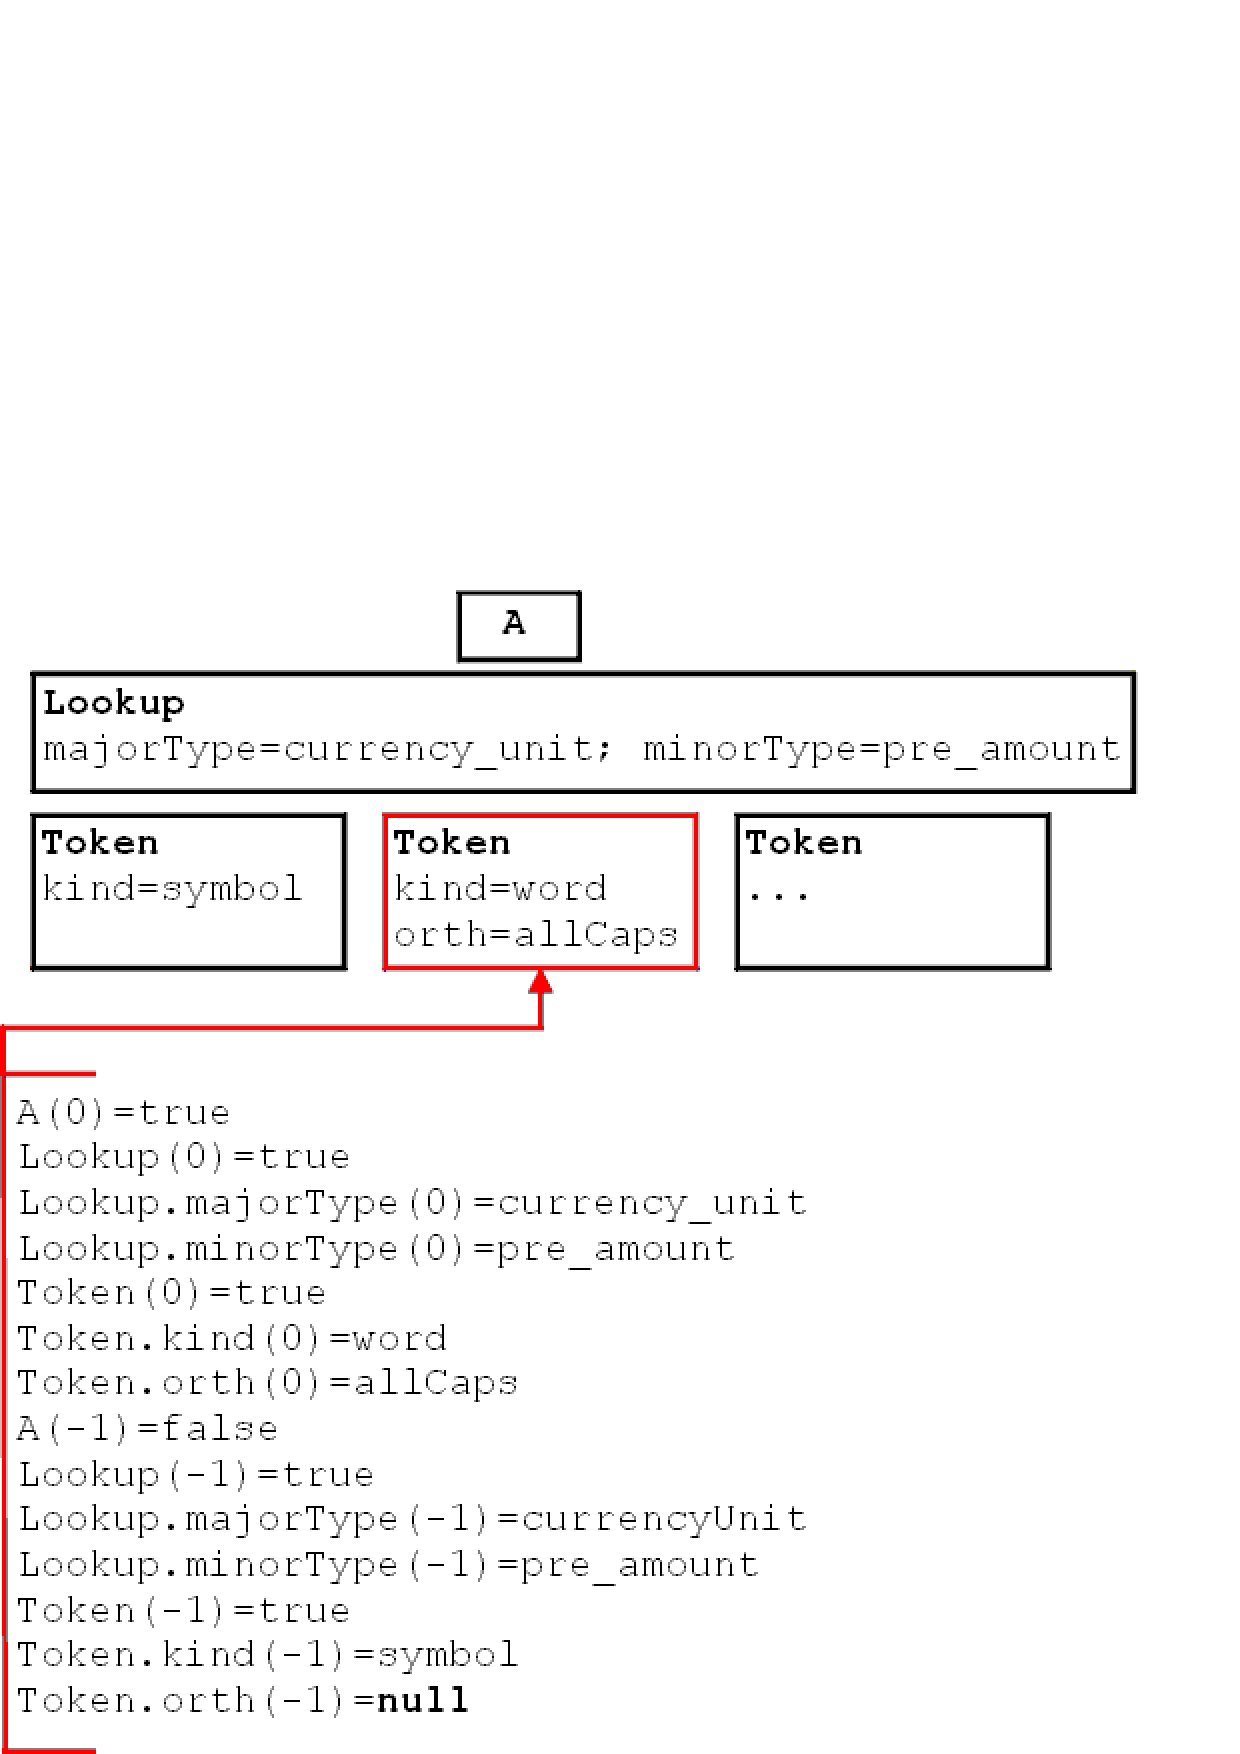
\includegraphics[scale=0.5]{attributes.png}
%\centerline{\epsfbox{scale=0.5}{attributes.eps}}
\end{center}
\caption{Sample attributes and their values}
\label{fig:attributes}
\end{figure}
%

An ATTRIBUTELIST element is similar to ATTRIBUTE except that it has no POSITION
sub-element but a RANGE element. This will be converted into several
ATTRIBUTELIST with position ranging from the value of the attribute `from' to
the value of the attribute `to'. This can be used in order to avoid the
duplication of ATTRIBUTE elements.

%%%%%%%%%%%%%%%%%%%%%%%%%%%%%%%%%%%%%%%%%%%%%%%%%%%%%%%%%%%%%%%%%%%%%%%%%%%%%
\subsect{The ENGINE Element}
%%%%%%%%%%%%%%%%%%%%%%%%%%%%%%%%%%%%%%%%%%%%%%%%%%%%%%%%%%%%%%%%%%%%%%%%%%%%%

The ENGINE element defines which particular ML implementation will be
used, and allows the setting of options for that particular
implementation.

The ENGINE element has three sub-elements:
\begin{itemize}
\item \textbf{WRAPPER}: defines the class name for the ML
implementation (or implementation wrapper). The specified class needs
to extend gate.creole.ml.MLEngine.

\item \textbf{BATCH-MODE-CLASSIFICATION}: this element is optional.  If present
(as an empty element \verb|<BATCH-MODE-CLASSIFICATION />|), the training
instances will be passed to the engine in a single batch.  If absent, the
instances are passed to the engine one at a time.  Not every engine supports
this option, but for those that do, it can greatly improve performance.

\item \textbf{OPTIONS}: the contents of the OPTIONS element will be
passed verbatim to the ML engine used.
\end{itemize}

%%%%%%%%%%%%%%%%%%%%%%%%%%%%%%%%%%%%%%%%%%%%%%%%%%%%%%%%%%%%%%%%%%%%%%%%%%%%%
\subsect{The WEKA Wrapper}
%%%%%%%%%%%%%%%%%%%%%%%%%%%%%%%%%%%%%%%%%%%%%%%%%%%%%%%%%%%%%%%%%%%%%%%%%%%%%

The PR provides a wrapper for the WEKA ML Library
(http://www.cs.waikato.ac.nz/ml/weka/) in the form of the
gate.creole.ml.weka.Wrapper class.

\subsubsect{Options for the WEKA Wrapper}

The WEKA wrapper accepts the following options:
\begin{itemize}
\item
\textbf{CLASSIFIER}: the class name for the classifier to be used.
\item
\textbf{CLASSIFIER-OPTIONS}: the options string as required for the
classifier.
\item
\textbf{CONFIDENCE-THRESHOLD}: a double value. If the classifier can
provide a probability distribution rather than a simple classification
then all possible classifications that have a probability value larger
or equal to the confidence threshold will be considered.
\item
\textbf{DATASET-FILE}: location of the weka arff file. This item is
not mandatory, it is possible to specify the file using the saving option on the
GUI.
\end{itemize}

\subsubsect{Training an ML Model with the WEKA Wrapper}

The Machine Learning PR has a Boolean runtime parameter named "training". When the
value of this parameter is set to true, the PR will collect a dataset
of instances from the documents on which it is run. If the classifier
used is an updatable classifier then the ML model will be built while
collecting the dataset. If the selected classifier is not updatable,
then the model will be built the first time a classification is
attempted.

Training a model consists of designing a definition file for the ML
PR, and creating an application containing a Machine Learning PR. When
the application is run over a corpus, the dataset (and the model if
possible) is built.

\subsubsect{Applying a Learnt Model}

Using the same PR, set the `training' parameter to false and run your
application.

Depending on the type of the attribute that is marked as class, different
actions will be performed when a classification occurs:
\begin{itemize}
\item if the attribute is boolean, a new annotation of the specified type
will be created with no features;
\item if the attribute is nominal or numeric, a new annotation of the
specified type will be created with the feature named in the attribute
definition having the value predicted by the classifier.
\end{itemize}

Once a model is learnt, it can be saved and reloaded at a later time.
The WEKA wrapper also provides an operation for saving only the dataset
in the ARFF format, which can be used for experiments in the WEKA
interface. This could be useful for determining the best algorithm to be
used and the optimal options for the selected algorithm.

%%%%%%%%%%%%%%%%%%%%%%%%%%%%%%%%%%%%%%%%%%%%%%%%%%%%%%%%%%%%%%%%%%%%%%%%%%%%%
\subsect[sec:ml:maxent]{The MAXENT Wrapper}
%%%%%%%%%%%%%%%%%%%%%%%%%%%%%%%%%%%%%%%%%%%%%%%%%%%%%%%%%%%%%%%%%%%%%%%%%%%%%

GATE also provides a wrapper for the Open NLP MAXENT library\\
(http://maxent.sourceforge.net/about.html). The MAXENT library provides an
implementation of the maximum entropy learning algorithm, and can be
accessed using the gate.creole.ml.maxent.MaxentWrapper class.

The MAXENT library requires all attributes except for the class
attribute to be boolean, and that the class attribute be boolean or nominal.
(It should be noted that, within maximum entropy terminology, the class
attribute is called the `outcome'.) Because the MAXENT library does not
provide a specific format for data sets, there is no facility to save or load
data sets separately from the model, but if there should be a need to do this,
the WEKA wrapper can be used to collect the data.

Training a MAXENT model follows the same general procedure as for WEKA models,
but the following difference should be noted. MAXENT models are not updateable,
so the model will always be created and trained the first time a classification
is attempted. The training of the model might take a considerable amount of time,
depending on the amount of training data and the parameters of the model.

\subsubsect{Options for the MAXENT Wrapper}

\begin{itemize}
\item
\textbf{CUT-OFF}: MAXENT features will only be included in the model if they occur
at least this many times. (The default value of this parameter is zero.)
\item
\textbf{ITERATIONS}: The number of times the training procedure should iterate when
finding the model's parameters (default is 10). In general no more than about 100
iterations should be needed to train a model, and it is recommended that less are
used during development to allow for shorter training times.
\item
\textbf{CONFIDENCE-THRESHOLD}: Same as for the WEKA wrapper (see above). However,
if this parameter is not set, or is set to zero, the model will not use a confidence
threshold, but will simply return the most likely classification.
\item
\textbf{SMOOTHING}: Use smoothing when training the model. Smoothing can improve
the accuracy of the learned models, but it will result in longer training times,
and training will use more memory. The size of the learned models will also be
larger. Generally smoothing will only improve performance for those models trained
from small data sets with a few outcomes. With larger data sets with lots of
outcomes, it may make performance worse.
\item
\textbf{SMOOTHING-OBSERVATION}: When using smoothing, this will specify the number
of times that trainer will imagine that it has seen features which it did not see
(default value is 0.1).
\item
\textbf{VERBOSE}: If selected, this will cause the classifier to output more
details of its operation during execution.
\end{itemize}

%%%%%%%%%%%%%%%%%%%%%%%%%%%%%%%%%%%%%%%%%%%%%%%%%%%%%%%%%%%%%%%%%%%%%%%%%%%%%
\subsect[sec:ml:svmlight]{The SVM Light Wrapper}
%%%%%%%%%%%%%%%%%%%%%%%%%%%%%%%%%%%%%%%%%%%%%%%%%%%%%%%%%%%%%%%%%%%%%%%%%%%%%

The PR provides a wrapper for the SVM Light ML system
(http://svmlight.joachims.org).  SVM Light is a support vector machine
implementation, written in C, which is provided as a set of command
line programs.  The wrapper takes care of the mundane work of
converting the data structures between GATE and SVM Light formats, and
calls the command line programs in the right sequence, passing the
data back and forth in temporary files.  The $<$WRAPPER$>$ value for
this engine is
\texttt{gate.creole.ml.svmlight.SVMLightWrapper}.

The SVM Light binaries themselves are not distributed with GATE -- you should
download the version for your platform from
\htlinkplain{http://svmlight.joachims.org} and place \texttt{svm\_learn} and
\texttt{svm\_classify} on your path.

Classifying documents using the SVMLightWrapper is a two phase procedure. In its
first phase, SVMWrapper collects data from the pre-annotated documents and
builds the SVM model using the collected data to classify the unseen documents
in its second phase. Below we describe briefly an example of classifying the
start time of the seminar in a corpus of email announcing seminars and provide
more details later in the section.

Figure \ref{fig:svmtrain} explains step by step the process of collecting
training data for the SVM classifier. GATE documents, which are pre-annotated
with the annotations of type \textit{Class} and feature \textit{type='stime'},
are used as the training data. In order to build the SVM model, we require start
and end annotations for each \textit{stime} annotation. We use a pre-processor
JAPE transduction script to mark the \textit{sTimeStart} and \textit{sTimeEnd}
annotations on \textit{stime} annotations. Following this step, the Machine
Learning PR (SVMLightWrapper) with training mode set to true collects the
training data from all training documents. A GATE corpus pipeline, given a set of
documents and PRs to execute on them, executes all PRs one by one, only on one
document at a time. Unless provided in a separate pipeline, it makes it
impossible to send all training data (i.e. collected from all documents)
altogether to the SVMWrapper using the same pipeline to build the SVM model.
This results in the model not being built at the time of collecting training
data. The state of the SVMWrapper can be saved to an external file once the
training data is collected.

\begin{figure}[h]
\center{\includegraphics[height=1.8cm]{SVMtrainning.png}}
\caption{Flow diagram explaining the SVM training data collection}
\label{fig:svmtrain}
\end{figure}

Before classifying any unseen document, SVM requires the SVM model to be
available. In the absence of an up-to-date SVM model, SVMWrapper builds a new
one using a command line \textit{SVM\_learn} utility and the training data
collected from the training corpus. In other words, the first SVM model is
built when a user tries to classify the first document. At this point the user
has an option to save the model somewhere. This is to enable reloading of the
model prior to classifying other documents and to avoid rebuilding of the SVM
model everytime the user classifies a new set of documents. Once the model
becomes available, SVMWrapper classifies the unseen documents which creates
new \textit{sTimeStart} and \textit{sTimeEnd} annotations over the text.
Finally, a post-processor JAPE transduction script is used to combine them
into the \textit{sTime} annotation. Figure \ref{fig:svmclassify} explains this
process.

\begin{figure}
\center{\includegraphics[height=8cm]{svmclassifier.png}}
\caption{Flow diagram explaining document classifying process}
\label{fig:svmclassify}
\end{figure}

The wrapper allows support vector machines to be created which do either
boolean classification or regression (estimation of numeric
parameters), and so the class attribute can be boolean or
numeric. Additionally, when learning a classifier, SVM Light
supports \emph{transduction}, whereby additional examples can be
presented during training which do not have the value of the class
attribute marked. Presenting such examples can, in some circumstances,
greatly improve the performance of the classifier. To make use of
this, the class attribute can be a three value nominal, in which case
the first value specified for that nominal in the configuration file
will be interpreted as
\emph{true}, the second as \emph{false} and the third as \emph{unknown}.
Transduction will be used with any instances for which this attribute
is set to the \emph{unknown} value. It is also possible to use a two
value nominal as the class attribute, in which case it will simply be
interpreted as \emph{true} or
\emph{false}.

The other attributes can be boolean, numeric or nominal, or any
combination of these. If an attribute is nominal, each value of that
attribute maps to a separate SVM Light feature. Each of these SVM
Light features will be given the value 1 when the nominal attribute
has the corresponding value, and will be omitted otherwise. If the
value of the nominal is not specified in the configuration file or
there is no value for an instance, then no feature will be added.

An extension to the basic functionality of SVM Light is that each
attribute can receive a weighting. These weighting can be specified in
the configuration file by adding \verb|<WEIGHTING>| tags to the parts
of the XML file specifying each attribute. The weighting for the
attribute must be specified as a numeric value, and be placed between
an opening \verb|<WEIGHTING>| tag and a closing
\verb|</WEIGHTING>| one. Giving an attribute a greater weighting, will cause it
to play a greater role in learning the model and classifying
data. This is achieved by multiplying the value of the attribute by
the weighting before creating the training or test data that is passed
to SVM Light. Any attribute left without an explicitly specified
weighting is given a default weighting of one. Support for these
weightings is contained in the Machine Learning PR itself, and so is
available to other wrappers, though at time of writing only the SVM
Light wrapper makes use of weightings.

As with the MAXENT wrapper, SVM Light models are not updateable, so
the model will be trained at the first classification attempt.  The
SVM Light wrapper supports \verb|<BATCH-MODE-CLASSIFICATION />|, which
should be used unless you have a very good reason not to.

The SVM Light wrapper allows both data sets and models to be loaded
and saved to files in the same formats as those used by SVM Light when
it is run from the command line. When a model is saved, a file will be
created which contains information about the state of the SVM Light
Wrapper, and which is needed to restore it when the model is loaded
again. This file does not, however, contain any information about the
SVM Light model itself. If an SVM Light model exists at the time of
saving, and that model is up to date with respect to the current state
of the training data, then it will be saved as a separate file, with
the same name as the file containing information about the state of
the wrapper, but with \texttt{.NativePart} appended to the
filename. These files are in the standard SVM Light model format, and
can be used with SVM Light when it is run from the command line. When
a model is reloaded by GATE, both of these files must be available,
and in the same directory, otherwise an error will result.  However,
if an up to date trained model does not exist at the time the model is
saved, then only one file will be created upon saving, and only that
file is required when the model is reloaded. So long as at least one
training instance exists, it is possible to bring the model up to date
at any point simply by classifying one or more instances (i.e. running
the model with the
\emph{training} parameter set to false).

\subsubsect{Options for the SVM Light Engine}
Only one \verb|<OPTIONS>| subelement is currently supported:
\begin{itemize}
\item \verb|<CLASSIFIER-OPTIONS>| a string of options to be passed to
\texttt{svm\_learn} on the command line. The only difference is that the user
should not specify whether regression or classification is to be used,
as the wrapper will detect this automatically, based on the type of
the class attribute, and set the option accordingly.
\end{itemize}

%%%%%%%%%%%%%%%%%%%%%%%%%%%%%%%%%%%%%%%%%%%%%%%%%%%%%%%%%%%%%%%%%%%%%%%%%%%%%
\subsect[sec:ml:ml-config]{Example Configuration File}
%%%%%%%%%%%%%%%%%%%%%%%%%%%%%%%%%%%%%%%%%%%%%%%%%%%%%%%%%%%%%%%%%%%%%%%%%%%%%

\scriptsize
\begin{verbatim}
<?xml version="1.0" encoding="UTF-8"?>
<ML-CONFIG>
  <DATASET>
  <!-- The type of annotation used as instance -->
  <INSTANCE-TYPE>Token</INSTANCE-TYPE>
  <ATTRIBUTE>
    <!-- The name given to the attribute -->
    <NAME>Lookup(0)</NAME>
    <!-- The type of annotation used as attribute -->
    <TYPE>Lookup</TYPE>
    <!-- The position relative to the instance annotation -->
    <POSITION>0</POSITION>
  </ATTRIBUTE>


  <ATTRIBUTE>
    <!-- The name given to the attribute -->
    <NAME>Lookup_MT(-1)</NAME>
    <!-- The type of annotation used as attribute -->
    <TYPE>Lookup</TYPE>
    <!-- Optional: the feature name for the feature used to extract values
    for the attribute -->
    <FEATURE>majorType</FEATURE>

    <!-- The position relative to the instance annotation -->
    <POSITION>-1</POSITION>
    <!-- The list of permitted values.
    if present, marks a nominal attribute;
    if absent, the attribute is numeric (double)        -->
    <VALUES>
      <!-- One permitted value -->
      <VALUE>address</VALUE>
      <VALUE>cdg</VALUE>
      <VALUE>country_adj</VALUE>
      <VALUE>currency_unit</VALUE>
      <VALUE>date</VALUE>
      <VALUE>date_key</VALUE>
      <VALUE>date_unit</VALUE>
      <VALUE>facility</VALUE>
      <VALUE>facility_key</VALUE>
      <VALUE>facility_key_ext</VALUE>
      <VALUE>govern_key</VALUE>
      <VALUE>greeting</VALUE>
      <VALUE>ident_key</VALUE>
      <VALUE>jobtitle</VALUE>
      <VALUE>loc_general_key</VALUE>
      <VALUE>loc_key</VALUE>
      <VALUE>location</VALUE>
      <VALUE>number</VALUE>
      <VALUE>org_base</VALUE>
      <VALUE>org_ending</VALUE>
      <VALUE>org_key</VALUE>
      <VALUE>org_pre</VALUE>
      <VALUE>organization</VALUE>
      <VALUE>organization_noun</VALUE>
      <VALUE>percent</VALUE>  
      <VALUE>person_ending</VALUE>
      <VALUE>person_first</VALUE>
      <VALUE>person_full</VALUE>
      <VALUE>phone_prefix</VALUE>
      <VALUE>sport</VALUE>
      <VALUE>spur</VALUE>
      <VALUE>spur_ident</VALUE>
      <VALUE>stop</VALUE>
      <VALUE>surname</VALUE>
      <VALUE>time</VALUE>
      <VALUE>time_modifier</VALUE>
      <VALUE>time_unit</VALUE>
      <VALUE>title</VALUE>
      <VALUE>year</VALUE>
    </VALUES>
    <!-- Optional: if present marks the attribute used as CLASS
    Only one attribute can be marked as class -->
  </ATTRIBUTE>

  <ATTRIBUTE>
    <!-- The name given to the attribute -->
    <NAME>Lookup_MT(0)</NAME>
    <!-- The type of annotation used as attribute -->
    <TYPE>Lookup</TYPE>
    <!-- Optional: the feature name for the feature used to extract values
    for the attribute -->
    <FEATURE>majorType</FEATURE>

    <!-- The position relative to the instance annotation -->
    <POSITION>0</POSITION>
    <!-- The list of permitted values.
    if present, marks a nominal attribute;
    if absent, the attribute is numeric (double)        -->
    <VALUES>
      <!-- One permitted value -->
          <VALUE>address</VALUE>
      <VALUE>cdg</VALUE>
      <VALUE>country_adj</VALUE>
      <VALUE>currency_unit</VALUE>
      <VALUE>date</VALUE>
      <VALUE>date_key</VALUE>
      <VALUE>date_unit</VALUE>
      <VALUE>facility</VALUE>
      <VALUE>facility_key</VALUE>
      <VALUE>facility_key_ext</VALUE>
      <VALUE>govern_key</VALUE>
      <VALUE>greeting</VALUE>
      <VALUE>ident_key</VALUE>
      <VALUE>jobtitle</VALUE>
      <VALUE>loc_general_key</VALUE>
      <VALUE>loc_key</VALUE>
      <VALUE>location</VALUE>
      <VALUE>number</VALUE>
      <VALUE>org_base</VALUE>
      <VALUE>org_ending</VALUE>
      <VALUE>org_key</VALUE>
      <VALUE>org_pre</VALUE>
      <VALUE>organization</VALUE>
      <VALUE>organization_noun</VALUE>
      <VALUE>percent</VALUE>  
      <VALUE>person_ending</VALUE>
      <VALUE>person_first</VALUE>
      <VALUE>person_full</VALUE>
      <VALUE>phone_prefix</VALUE>
      <VALUE>sport</VALUE>
      <VALUE>spur</VALUE>
      <VALUE>spur_ident</VALUE>
      <VALUE>stop</VALUE>
      <VALUE>surname</VALUE>
      <VALUE>time</VALUE>
      <VALUE>time_modifier</VALUE>
      <VALUE>time_unit</VALUE>
      <VALUE>title</VALUE>
      <VALUE>year</VALUE>
    </VALUES>
    <!-- Optional: if present marks the attribute used as CLASS
    Only one attribute can be marked as class -->
  </ATTRIBUTE>

  <ATTRIBUTE>
    <!-- The name given to the attribute -->
    <NAME>Lookup_MT(1)</NAME>
    <!-- The type of annotation used as attribute -->
    <TYPE>Lookup</TYPE>
    <!-- Optional: the feature name for the feature used to extract values
    for the attribute -->
    <FEATURE>majorType</FEATURE>

    <!-- The position relative to the instance annotation -->
    <POSITION>1</POSITION>

    <!-- The list of permitted values.
    if present, marks a nominal attribute;
    if absent, the attribute is numeric (double)        -->
    <VALUES>
      <!-- One permitted value -->
      <VALUE>address</VALUE>
      <VALUE>cdg</VALUE>
      <VALUE>country_adj</VALUE>
      <VALUE>currency_unit</VALUE>
      <VALUE>date</VALUE>
      <VALUE>date_key</VALUE>
      <VALUE>date_unit</VALUE>
      <VALUE>facility</VALUE>
      <VALUE>facility_key</VALUE>
      <VALUE>facility_key_ext</VALUE>
      <VALUE>govern_key</VALUE>
      <VALUE>greeting</VALUE>
      <VALUE>ident_key</VALUE>
      <VALUE>jobtitle</VALUE>
      <VALUE>loc_general_key</VALUE>
      <VALUE>loc_key</VALUE>
      <VALUE>location</VALUE>
      <VALUE>number</VALUE>
      <VALUE>org_base</VALUE>
      <VALUE>org_ending</VALUE>
      <VALUE>org_key</VALUE>
      <VALUE>org_pre</VALUE>
      <VALUE>organization</VALUE>
      <VALUE>organization_noun</VALUE>
      <VALUE>percent</VALUE>  
      <VALUE>person_ending</VALUE>
      <VALUE>person_first</VALUE>
      <VALUE>person_full</VALUE>
      <VALUE>phone_prefix</VALUE>
      <VALUE>sport</VALUE>
      <VALUE>spur</VALUE>
      <VALUE>spur_ident</VALUE>
      <VALUE>stop</VALUE>
      <VALUE>surname</VALUE>
      <VALUE>time</VALUE>
      <VALUE>time_modifier</VALUE>
      <VALUE>time_unit</VALUE>
      <VALUE>title</VALUE>
      <VALUE>year</VALUE>
    </VALUES>
    <!-- Optional: if present marks the attribute used as CLASS
    Only one attribute can be marked as class -->
  </ATTRIBUTE>

  <ATTRIBUTE>
    <!-- The name given to the attribute -->
    <NAME>POS_category(-1)</NAME>
    <!-- The type of annotation used as attribute -->
    <TYPE>Token</TYPE>
    <!-- Optional: the feature name for the feature used to extract values
    for the attribute -->
    <FEATURE>category</FEATURE>

    <!-- The position relative to the instance annotation -->
    <POSITION>-1</POSITION>

    <!-- The list of permitted values.
    if present, marks a nominal attribute;
    if absent, the attribute is numeric (double)        -->
    <VALUES>
      <!-- One permitted value -->
        <VALUE>NN</VALUE>
        <VALUE>NNP</VALUE>
        <VALUE>NNPS</VALUE>
        <VALUE>NNS</VALUE>
        <VALUE>NP</VALUE>
        <VALUE>NPS</VALUE>
        <VALUE>JJ</VALUE>
        <VALUE>JJR</VALUE>
        <VALUE>JJS</VALUE>
        <VALUE>JJSS</VALUE>
        <VALUE>RB</VALUE>
        <VALUE>RBR</VALUE>
        <VALUE>RBS</VALUE>
        <VALUE>VB</VALUE>
        <VALUE>VBD</VALUE>
        <VALUE>VBG</VALUE>
        <VALUE>VBN</VALUE>
        <VALUE>VBP</VALUE>
        <VALUE>VBZ</VALUE>
        <VALUE>FW</VALUE>
        <VALUE>CD</VALUE>
        <VALUE>CC</VALUE>
        <VALUE>DT</VALUE>
        <VALUE>EX</VALUE>
        <VALUE>IN</VALUE>
        <VALUE>LS</VALUE>
        <VALUE>MD</VALUE>
        <VALUE>PDT</VALUE>
        <VALUE>POS</VALUE>
        <VALUE>PP</VALUE>
        <VALUE>PRP</VALUE>
        <VALUE>PRP$</VALUE>
        <VALUE>PRPR$</VALUE>
        <VALUE>RP</VALUE>
        <VALUE>TO</VALUE>
        <VALUE>UH</VALUE>
        <VALUE>WDT</VALUE>
        <VALUE>WP</VALUE>
        <VALUE>WP$</VALUE>
        <VALUE>WRB</VALUE>
        <VALUE>SYM</VALUE>
        <VALUE>\"</VALUE>
        <VALUE>#</VALUE>
        <VALUE>$</VALUE>
        <VALUE>'</VALUE>
        <VALUE>(</VALUE>
        <VALUE>)</VALUE>
        <VALUE>,</VALUE>
        <VALUE>--</VALUE>
        <VALUE>-LRB-</VALUE>
        <VALUE>.</VALUE>
        <VALUE>''</VALUE>
        <VALUE>:</VALUE>
        <VALUE>::</VALUE>
        <VALUE>`</VALUE>
    </VALUES>
    <!-- Optional: if present marks the attribute used as CLASS
    Only one attribute can be marked as class -->
  </ATTRIBUTE>

  <ATTRIBUTE>
    <!-- The name given to the attribute -->
    <NAME>POS_category(0)</NAME>
    <!-- The type of annotation used as attribute -->
    <TYPE>Token</TYPE>
    <!-- Optional: the feature name for the feature used to extract values
    for the attribute -->
    <FEATURE>category</FEATURE>

    <!-- The position relative to the instance annotation -->
    <POSITION>0</POSITION>

    <!-- The list of permitted values.
    if present, marks a nominal attribute;
    if absent, the attribute is numeric (double)        -->
    <VALUES>
      <!-- One permitted value -->
        <VALUE>NN</VALUE>
        <VALUE>NNP</VALUE>
        <VALUE>NNPS</VALUE>
        <VALUE>NNS</VALUE>
        <VALUE>NP</VALUE>
        <VALUE>NPS</VALUE>
        <VALUE>JJ</VALUE>
        <VALUE>JJR</VALUE>
        <VALUE>JJS</VALUE>
        <VALUE>JJSS</VALUE>
        <VALUE>RB</VALUE>
        <VALUE>RBR</VALUE>
        <VALUE>RBS</VALUE>
        <VALUE>VB</VALUE>
        <VALUE>VBD</VALUE>
        <VALUE>VBG</VALUE>
        <VALUE>VBN</VALUE>
        <VALUE>VBP</VALUE>
        <VALUE>VBZ</VALUE>
        <VALUE>FW</VALUE>
        <VALUE>CD</VALUE>
        <VALUE>CC</VALUE>
        <VALUE>DT</VALUE>
        <VALUE>EX</VALUE>
        <VALUE>IN</VALUE>
        <VALUE>LS</VALUE>
        <VALUE>MD</VALUE>
        <VALUE>PDT</VALUE>
        <VALUE>POS</VALUE>
        <VALUE>PP</VALUE>
        <VALUE>PRP</VALUE>
        <VALUE>PRP$</VALUE>
        <VALUE>PRPR$</VALUE>
        <VALUE>RP</VALUE>
        <VALUE>TO</VALUE>
        <VALUE>UH</VALUE>
        <VALUE>WDT</VALUE>
        <VALUE>WP</VALUE>
        <VALUE>WP$</VALUE>
        <VALUE>WRB</VALUE>
        <VALUE>SYM</VALUE>
        <VALUE>\"</VALUE>
        <VALUE>#</VALUE>
        <VALUE>$</VALUE>
        <VALUE>'</VALUE>
        <VALUE>(</VALUE>
        <VALUE>)</VALUE>
        <VALUE>,</VALUE>
        <VALUE>--</VALUE>
        <VALUE>-LRB-</VALUE>
        <VALUE>.</VALUE>
        <VALUE>''</VALUE>
        <VALUE>:</VALUE>
        <VALUE>::</VALUE>
        <VALUE>`</VALUE>
    </VALUES>
    <!-- Optional: if present marks the attribute used as CLASS
    Only one attribute can be marked as class -->
  </ATTRIBUTE>

  <ATTRIBUTE>
    <!-- The name given to the attribute -->
    <NAME>POS_category(1)</NAME>
    <!-- The type of annotation used as attribute -->
    <TYPE>Token</TYPE>
    <!-- Optional: the feature name for the feature used to extract values
    for the attribute -->
    <FEATURE>category</FEATURE>

    <!-- The position relative to the instance annotation -->
    <POSITION>1</POSITION>

    <!-- The list of permitted values.
    if present, marks a nominal attribute;
    if absent, the attribute is numeric (double)        -->
    <VALUES>
      <!-- One permitted value -->
        <VALUE>NN</VALUE>
        <VALUE>NNP</VALUE>
        <VALUE>NNPS</VALUE>
        <VALUE>NNS</VALUE>
        <VALUE>NP</VALUE>
        <VALUE>NPS</VALUE>
        <VALUE>JJ</VALUE>
        <VALUE>JJR</VALUE>
        <VALUE>JJS</VALUE>
        <VALUE>JJSS</VALUE>
        <VALUE>RB</VALUE>
        <VALUE>RBR</VALUE>
        <VALUE>RBS</VALUE>
        <VALUE>VB</VALUE>
        <VALUE>VBD</VALUE>
        <VALUE>VBG</VALUE>
        <VALUE>VBN</VALUE>
        <VALUE>VBP</VALUE>
        <VALUE>VBZ</VALUE>
        <VALUE>FW</VALUE>
        <VALUE>CD</VALUE>
        <VALUE>CC</VALUE>
        <VALUE>DT</VALUE>
        <VALUE>EX</VALUE>
        <VALUE>IN</VALUE>
        <VALUE>LS</VALUE>
        <VALUE>MD</VALUE>
        <VALUE>PDT</VALUE>
        <VALUE>POS</VALUE>
        <VALUE>PP</VALUE>
        <VALUE>PRP</VALUE>
        <VALUE>PRP$</VALUE>
        <VALUE>PRPR$</VALUE>
        <VALUE>RP</VALUE>
        <VALUE>TO</VALUE>
        <VALUE>UH</VALUE>
        <VALUE>WDT</VALUE>
        <VALUE>WP</VALUE>
        <VALUE>WP$</VALUE>
        <VALUE>WRB</VALUE>
        <VALUE>SYM</VALUE>
        <VALUE>\"</VALUE>
        <VALUE>#</VALUE>
        <VALUE>$</VALUE>
        <VALUE>'</VALUE>
        <VALUE>(</VALUE>
        <VALUE>)</VALUE>
        <VALUE>,</VALUE>
        <VALUE>--</VALUE>
        <VALUE>-LRB-</VALUE>
        <VALUE>.</VALUE>
        <VALUE>''</VALUE>
        <VALUE>:</VALUE>
        <VALUE>::</VALUE>
        <VALUE>`</VALUE>
    </VALUES>
    <!-- Optional: if present marks the attribute used as CLASS
    Only one attribute can be marked as class -->
  </ATTRIBUTE>

  <ATTRIBUTE>
    <!-- The name given to the attribute -->
    <NAME>Entity(0)</NAME>
    <!-- The type of annotation used as attribute -->
    <TYPE>Entity</TYPE>
    <!-- The position relative to the instance annotation -->
    <POSITION>0</POSITION>

    <CLASS/>
    <!-- Optional: if present marks the attribute used as CLASS
    Only one attribute can be marked as class -->
  </ATTRIBUTE>


  </DATASET>

  <ENGINE>
    <WRAPPER>gate.creole.ml.weka.Wrapper</WRAPPER>
    <OPTIONS>
        <CLASSIFIER OPTIONS="-S -C 0.25 -B -M 2">weka.classifiers.trees.J48</CLASSIFIER>
        <CONFIDENCE-THRESHOLD>0.85</CONFIDENCE-THRESHOLD>
    </OPTIONS>
  </ENGINE>
</ML-CONFIG>
\end{verbatim}
\normalsize
